\documentclass[UTF8, xcolor=table]{beamer}

% 定义本文所使用宏包
% !Mode:: "TeX:UTF-8"

% 原作者信息Original Authors:
% 张井   Jing Zhang: prayever@gmail.com     天津大学2010级管理与经济学部信息管理与信息系统专业硕士生
% 余蓝涛 Lantao Yu: lantaoyu1991@gmail.com  天津大学2008级精密仪器与光电子工程学院测控技术与仪器专业本科生

% Thanks 中大移植版by林海涛&徐浩晖&

%%%%%%%%%% Package %%%%%%%%%%%%

% 支持插图处理
\usepackage{graphicx}
% 控制文档布局
%\usepackage[a4paper,text={146.4 true mm,239.2 true mm},top= 26.2 true mm,left=31.8 true mm,head=6 true mm,headsep=6.5 true mm,foot=16.5 true mm]{geometry}
\usepackage[a4paper,text={146.4 true mm,239.2 true mm},top= 26.2 true mm,left=31.8 true mm,head=6 true mm,headsep=6.5 true mm,foot=16.5 true mm,footnotesep=-8 true mm]{geometry}

% 支持版面尺寸设置
% 支持国际标准单位
\usepackage[squaren]{SIunits}               

\usepackage{titletoc}                       % 控制目录的宏包
\usepackage[raggedleft]{titlesec}               % 控制标题的宏包

\usepackage{fancyhdr}                       % fancyhdr宏包 支持页眉和页脚的相关定义

\usepackage[UTF8]{ctex}                     % 支持中文显示
\usepackage{color}                          % 支持彩色
\usepackage{amsmath}                        % AMSLaTeX宏包 用来排出更加漂亮的公式
\usepackage{amssymb}                        % 数学符号生成命令
\usepackage[below]{placeins}    %允许上一个section的浮动图形出现在下一个section的开始部分,还提供\FloatBarrier命令,使所有未处理的浮动图形立即被处理
\usepackage{multirow}                       % 使用Multirow宏包,使得表格可以合并多个row格
\usepackage{booktabs}                       % 表格,横的粗线;\specialrule{1pt}{0pt}{0pt}
\usepackage{longtable}                      % 支持跨页的表格。
\usepackage{tabularx}                       % 自动设置表格的列宽
\usepackage{diagbox}						% 制作斜线单元格
\usepackage{makecell}

%\usepackage{subfigure}                      % 支持子图 %centerlast 设置最后一行是否居中
%\usepackage[subfigure]{ccaption}            % 支持子图的中文标题
% use the more updated subcaption package, which has replaced subfigure
\usepackage{subcaption}
%\usepackage{caption}
%\usepackage{capt-of}

\usepackage{dsfont}                         % 支持空心数字

\usepackage[sort&compress,numbers]{natbib}  % 支持引用缩写的宏包
\usepackage{enumitem}                       % 使用enumitem宏包,改变列表项的格式
\usepackage{calc}                           % 长度可以用+ - * / 进行计算
\usepackage{txfonts}                        % 字体宏包
\usepackage{bm}                             % 处理数学公式中的黑斜体的宏包
\usepackage[amsmath,thmmarks,hyperref]{ntheorem}  % 定理类环境宏包,其中 amsmath 选项用来兼容 AMS LaTeX 的宏包
\usepackage{CJKnumb}                        % 提供将阿拉伯数字转换成中文数字的命令
\usepackage{indentfirst}                    % 首行缩进宏包
%\usepackage{hypbmsec}                      % 用来控制书签中标题显示内容
\newcommand{\tabincell}[2]{\begin{tabular}{@{}#1@{}}#2\end{tabular}}
\usepackage{xcolor}
% 支持代码环境
\usepackage{listings}
\lstset{numbers=left,
	language=[ANSI]{C},
	numberstyle=\tiny,
	extendedchars=false,
	showstringspaces=false,
	breakatwhitespace=false,
	breaklines=true,
	captionpos=b,
	keywordstyle=\color{blue!70},
	commentstyle=\color{red!50!green!50!blue!50},
	frame=shadowbox,
	rulesepcolor=\color{red!20!green!20!blue!20}
}
% 支持算法环境
\usepackage{algpseudocode}
\usepackage[linesnumbered,ruled,vlined]{algorithm2e}
%\usepackage{algorithmic}
%\usepackage{algorithm,algpseudocode}

\usepackage{array}
\newcommand{\PreserveBackslash}[1]{\let\temp=\\#1\let\\=\temp}
\newcolumntype{C}[1]{>{\PreserveBackslash\centering}p{#1}}
\newcolumntype{R}[1]{>{\PreserveBackslash\raggedleft}p{#1}}
\newcolumntype{L}[1]{>{\PreserveBackslash\raggedright}p{#1}}

% 生成有书签的 pdf 及其生成方式。通常可以在 tjumain.tex 文件的第一行选择 pdflatex 或者是 dvipdfmx 编译手段。如果选择前者,则使用 pdflatex + pdflatex 编译; 如果选择后者,在编译的时候选择 latex + bibtex + latex + latex 编译。出现混淆的时候,系统会报错。
% 如果您的pdf制作中文书签有乱码使用如下命令,就可以解决了
\def\atemp{dvipdfmx}\ifx\atemp\usewhat
\usepackage[dvipdfmx,unicode,               % dvipdfmx 编译, 加入了中文复制,粘贴支持引擎。
            pdfstartview=FitH,
            bookmarksnumbered=true,
            bookmarksopen=true,
            colorlinks=false,
            pdfborder={0 0 1},
            citecolor=blue,
            linkcolor=red,
            anchorcolor=green,
            urlcolor=blue,
            breaklinks=true
            ]{hyperref}
\fi

\def\atemp{pdflatex}\ifx\atemp\usewhat
\usepackage{cmap}                           % pdflatex 编译时,可以生成可复制、粘贴的中文 PDF 文档, 缺点是在Windows上显示时效果不大好,字体发虚
\usepackage[pdftex,unicode,
            %CJKbookmarks=true,
            bookmarksnumbered=true,
            bookmarksopen=true,				
            hidelinks
%            colorlinks=true,		% original false
%            pdfborder={0 0 1},
%            citecolor=black,		% original blue
%            linkcolor=black,		% original red
%            anchorcolor=black,		% original green
%            urlcolor=blue,
%            breaklinks=false		% original true
            ]{hyperref}
\fi

% 新增for url
\usepackage{url}

% \pdfbookmark and \tableofcontents
\usepackage[bookmarks=true]{hyperref}
\usepackage{bookmark}

% xeCJK直接使用Window系统字体(一定要保证tex所存格式为UTF8,否则xeCJK汉字不显示)
\usepackage{xeCJK}
\usepackage{etoolbox}

% 控制打印模式
\usepackage{ifthen}
% 脚注跨章连续编号
%\usepackage{chngcntr}
% 脚注按页单独编号
\usepackage[perpage]{footmisc}
% \includepdf{}
\usepackage{pdfpages}

\graphicspath{{./figures/}}

\begin{document}
	\setbeamerfont{footnote}{size=\tiny}
	\setbeamerfont{caption}{size=\scriptsize}
	\setbeamertemplate{caption}[numbered]
	\setbeamerfont{subsection in toc}{size=\footnotesize}
	\renewcommand*{\bibfont}{\footnotesize}
	
	\title[融合长短记忆神经网络与卷积特征学习的图像语义分割]{中文题目 \\ \vskip 8pt \normalsize The English Title \\ Title...}
	\author[~~~~陈胜杰~~~~CHEN Shengjie]{}
	\institute[中山大学~数据科学与计算机学院~工程硕士(软件工程)]{}
	\date{}
	
	%% make title %%
	{
		\setbeamertemplate{headline}{}
		\setbeamertemplate{footline}{}
		
		\usebackgroundtemplate{%
			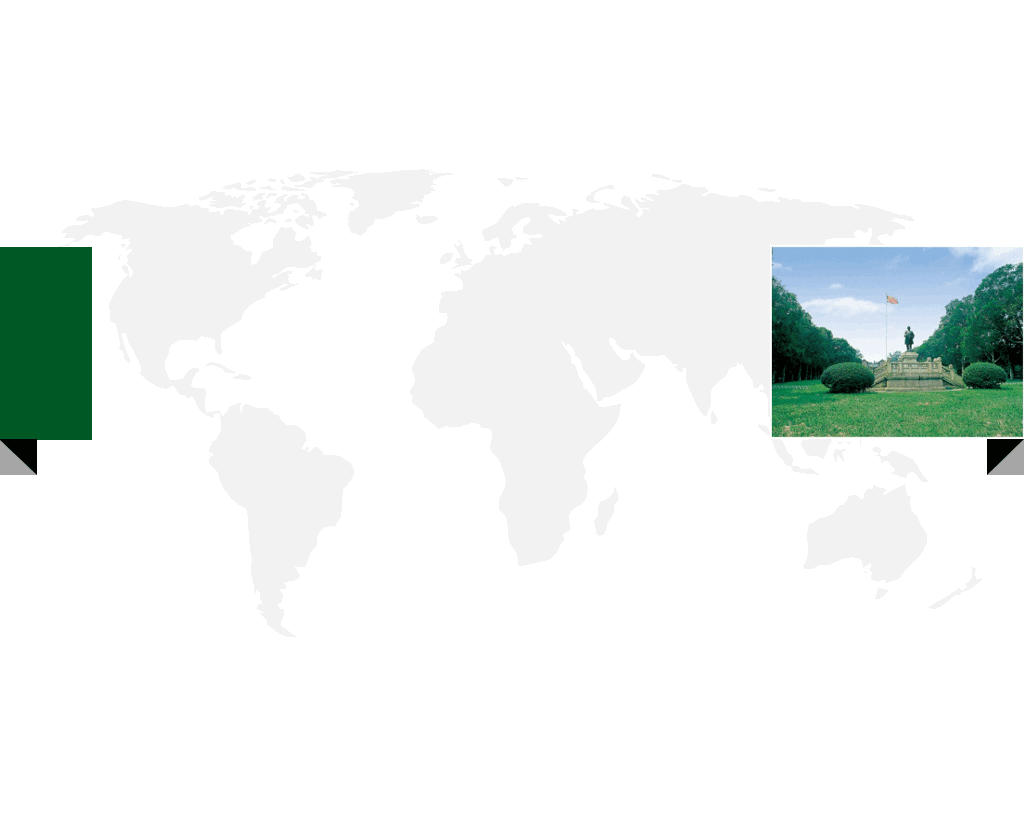
\includegraphics[width=\paperwidth,height=\paperheight]{styles/title.png}
		}
		
		\begin{frame}
		%\begin{frame}[plain]
			%% make logo without name %%
			%\begin{flushright}
			%	\vspace{-15mm}
			%	
\includegraphics[width=1.48cm]{styles/badge.png}
			%\end{flushright}
			
			%% make logo with name %%
			\begin{flushright}
				\vspace{-13.888mm}
				
\includegraphics[width=4.5cm]{styles/logo.png}
			\end{flushright}
		
			\vspace{-7.888mm}
			\titlepage
			
			\begin{flushright}
				\begin{tabular}{lc}
					学位申请人   &  \underline{\makebox[108pt][c]{陈胜杰}} \\
					专\ 业\ 名\ 称   &  \underline{\makebox[108pt][c]{工程硕士(软件工程)}} \\
					答\ 辩\ 时\ 间   &  \underline{\makebox[108pt][c]{May 13, 2018}} \\
				\end{tabular}
			\end{flushright}
		\end{frame}
	}
	\addtocounter{framenumber}{-1}
	
	%% make contents %%
	\frame {
		\frametitle{目录}
		\tableofcontents[sections={<1-7>}]
	}

	%% make body %%
	% !Mode:: "TeX:UTF-8"
\chapter{引言}
\label{ch:intro}
本章主要介绍了自动驾驶的技术背景以及三维物体检测在自动驾驶技术中的重要作用,然后引出了目前三维物体检测技术的局限性。之后,本章介绍了目前国内外对三维物体检测的研究进展,也简单介绍了三维多目标追踪的研究进展。最后,本章简要概括了本文的工作重点以及技术创新要点,强调了本文研究对于自动驾驶领域的重要意义。

\section{研究背景与意义}
\label{sec:background}
近几年来, 深度学习的迅猛发展赋予了机器越来越强的智能。在计算机视觉、自然语言处理等领域的某些任务上,机器甚至能够表现出比人类更好的性能\cite{he2016deep,DevlinBERT}。 在这样的大背景下, 无人驾驶(Autonomous Driving) 作为最能够体现机器智能的应用场景之一,受到了学术界和工业界的广泛关注。 无人驾驶要求机器能够像人类一样识别道路场景,包括行人和车辆的状态以及车道线等,并且能够根据这些信息高效地进行路径规划来实现与人类类似的驾驶行为。 无人驾驶应用十分广泛,无论是民用还是军工领域。 机器取代人类驾驶车辆,一方面能让人们出行效率更高, 另一方面,机器之间的通讯比人类效率更高,这使得车辆能够更好的规划自己的行驶路径,降低交通事故发生概率。作为智慧城市的不可缺少的组成部分, 无人驾驶也能在非常时期发挥重要作用。譬如在面对重大传染病时(如2019年末爆发的COVID-19),人员之间要尽量减少接触,此时无人驾驶能在保证安全的情况下,极大方便人们的日常生活,包括出行以及货物配送。因此,无人驾驶作为可预见的未来技术,一直是各国在高科技领域的“必争之地”。近十几年来,国内外的无人驾驶平台如雨后春笋般冒出,既有老牌互联网大公司开展的新业务,如国内百度的Apollo\footnote[1]{http://apollo.auto/}(如\figurename \ref{fig:apollo}),美国Google的Waymo\footnote[2]{https://waymo.com/}(如\figurename \ref{fig:waymo})等;也有新型汽车行业巨头,如Uber、特斯拉、滴滴、上汽等;另外,还有新兴的无人驾驶创业公司,如pony.ai、图森未来、驭势科技等。这些都是推动无人驾驶商业化不可忽视的力量,也是推动无人驾驶技术落地的中坚力量。

\begin{figure}[!t]
	\centering
	\begin{minipage}[t]{0.40\textwidth}
		\centering
		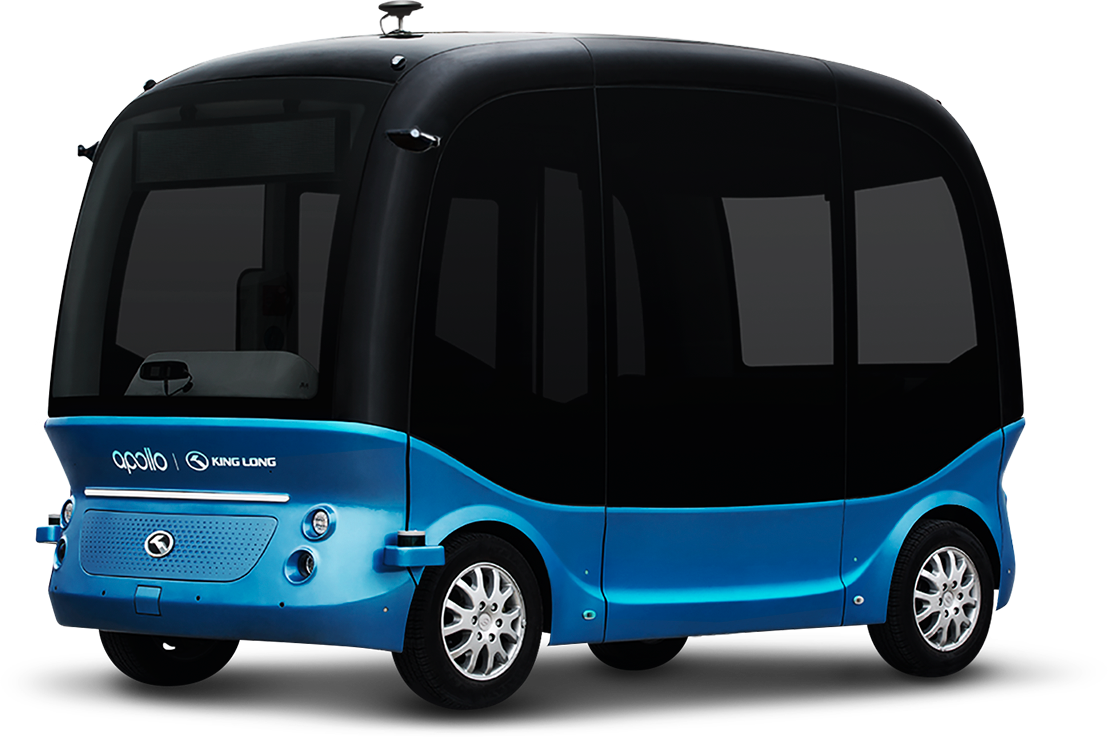
\includegraphics[width=\textwidth]{./imgs/apollo.png}
		\caption{Apollo自动驾驶汽车}
		\label{fig:apollo}
	\end{minipage}
	\begin{minipage}[t]{0.55\textwidth}
		\centering
		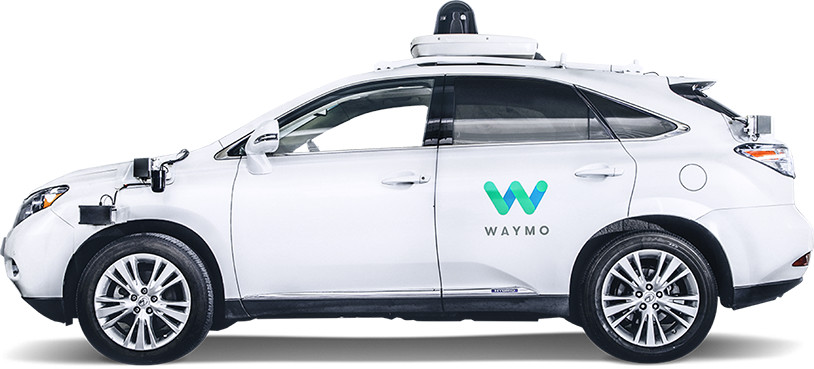
\includegraphics[width=\textwidth]{./imgs/waymo.jpg}
		\caption{Waymo自动驾驶汽车}
		\label{fig:waymo}
	\end{minipage}
\end{figure}


无人驾驶技术主要包括感知、决策和规划三个重要模块,其中感知模块是无人驾驶技术的基础,也是难点。感知模块的任务是赋予机器理解环境的能力,使机器能够准确捕获复杂道路场景的有用信息。目前无人驾驶车辆依赖多种传感器感知环境, 譬如激光雷达(LIDAR)、摄像头、毫米波雷达等。这些传感器都有着各自的优缺点,特别是在价格、使用场景以及探测距离方面,如表\ref{table:sensor_cmp}所示。因此,目前绝大多数自动驾驶公司在感知模块都使用多传感器融合技术,让各传感器优劣互补。多传感器采集的数据会通过算法进行融合,尽可能准确的还原真实的三维环境信息,以便用于后续的目标检测以及跟踪等任务。

环境感知中一大核心任务是物体检测(Object Detection), 即通过分析传感器采集的数据,确定环境中各目标的位姿,包括其在世界坐标系下的坐标、形状信息以及朝向。不同于以图像为主要数据载体的二维物体检测,自动驾驶领域的物体检测任务要求预测目标在三维空间的位姿信息,即三维目标检测。三维目标检测比二维目标检测更加具有挑战性,这是因为维度诅咒(the curse of dimensionality)的存在: 当维度增加时,空间的体积增加的非常之快(以指数增加),以致于可用的数据变得稀疏。 三维物体检测的一大挑战,就是三维数据的稀疏性。目前无人驾驶中三维数据的获得主要是依靠激光雷达,其原理是通过高速旋转的激光发射器向周围发射激光,然后检测接收到反射回来光线的时间间隔来计算反射点的距离。激光雷达的线束对其分辨率有很大影响,特别是对于远距离的目标,在低线束(例如16线)激光雷达中可能只有稀疏的几个点,完全无法分辨。而分辨率高的高线束的激光雷达则十分昂贵,以 Velodyne 64线激光雷达为例,其价格高达十几万美金,因此多数无人驾驶技术方案都需要在激光雷达分辨率与价格之间做出权衡。最近一种非完全旋转的激光雷达——固态激光雷达\footnote[3]{http://www.robosense.cn/rslidar/rs-lidar-m1}受到越来越多人的关注,它们具备数据采集速度快、分辨率高、价格低廉以及环境适应性强等特点,被自动驾驶行业给予厚望。然而目前该技术尚不成熟,还没经过广泛的实际场景检验,离落地还有一段时间,因此暂时不在各大方案的候选传感器之内。短期来看,传统的机械式激光雷达仍是各大自动驾驶平台的首选。

\begin{table}
	\centering
	\wuhao
	\caption{自动驾驶各传感器对比\cite{FirstAVbook}。}
	\vspace{0.3cm}
	\resizebox{\textwidth}{!}{
		\begin{tabular}{cccccccc}
			\toprule[1.5pt]
			传感器    & 激光雷达(LIDAR) & 摄像头(Camera) & 毫米波雷达 \\ \midrule
			外形      & \begin{minipage}{0.13\textwidth}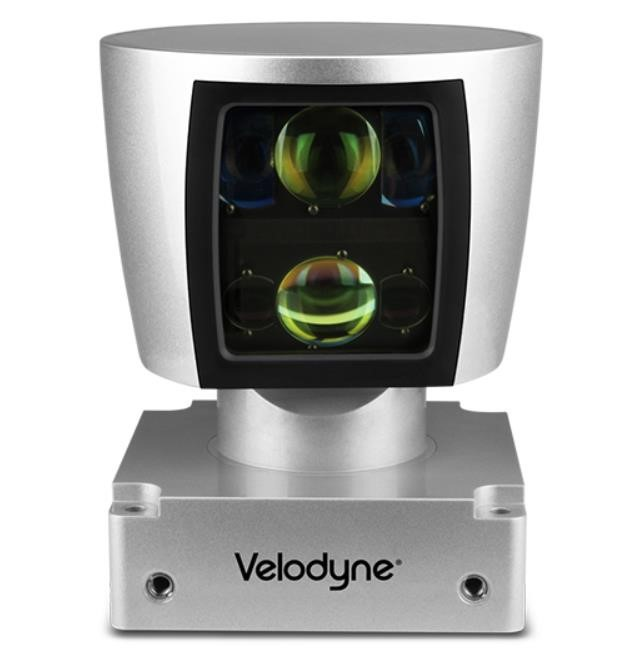
\includegraphics[width=\linewidth]{../figures/imgs/lidar.jpg}\end{minipage} & \begin{minipage}{0.15\textwidth}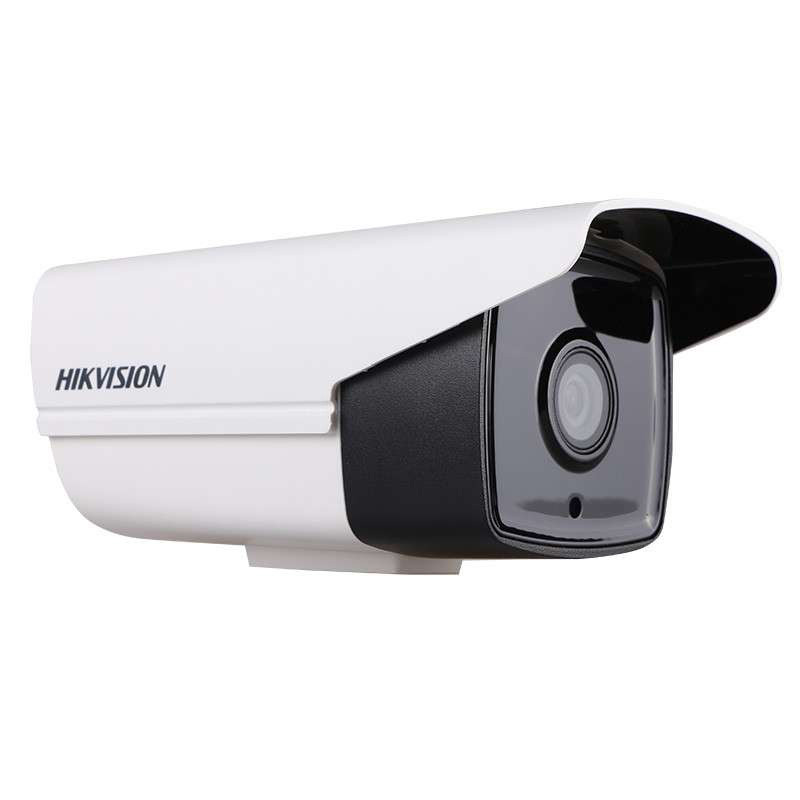
\includegraphics[width=\linewidth]{../figures/imgs/camera.jpg}\end{minipage} & \begin{minipage}{0.15\textwidth}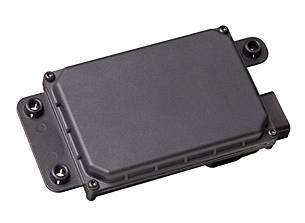
\includegraphics[width=\linewidth]{../figures/imgs/mlidar.jpeg}\end{minipage} \\ \hline
			价格      & 8000美元以上    & 35-50美元         & 300-500美元    \\ \hline
			优点      & \makecell*[c]{扫描周围环境得到精确\\环境信息、距离信息}   & \makecell*[c]{成本比较低,通过算法\\可以实现各种功能} & \makecell*[c]{不受天气影响,\\测量精度高}  \\ \hline
			缺点      & \makecell*[c]{成本高,大雾、雨雪天气\\效果差,无法图像识别}  & \makecell*[c]{恶劣环境下失效,难以测距,\\探测距离较近,算法要求高}   & \makecell*[c]{无法识别道路指示牌,\\无法识别行人}   \\ 
			\bottomrule[1.5pt]
	\end{tabular}}
	\label{table:sensor_cmp}
\end{table}


根据使用传感器数据的不同,目前三维物体检测的研究主要有三个方向:基于图像数据的方案\cite{7780605, chen20183d},基于点云数据的方案\cite{li20173d,engelcke2017vote3deep,zhou2018voxelnet,simon2018complex,shi2019pointrcnn},以及基于多传感器数据融合的方案\cite{qi2018frustum,chen2017multi,ku2018joint}。借助深度学习技术,这些方案都取得了很不错的结果。尽管如此,目前基本所有的三维物体检测方案都是针对单帧数据进行检测。对于真实的自动驾驶场景的物体检测任务来说,数据都是以流的形式连续获取的。从算法落地的难易程度方面考虑,开发针对流数据的三维物体检测算法相比于基于单帧的三维物体检查算法更加具有优势。相比于单帧数据,流数据可以提供同一目标在一段时间内的连续信息。一方面,由于检测噪声(误检测的物体)在时间维度上连续性较差,因此时序上的连续信息有利于检测算法筛除误检测的目标。另一方面,对于遮挡以及物体框被边界截断的目标,在流数据中可以利用前后帧的信息对其进行补全,从而获得更好的检测性能,这对于基于单帧的检测算法来说是难以实现的。最后值得注意的是,流数据一般有很强的数据冗余性,即相邻帧之间绝大多数信息都相同,只有存在物体运动的区域才会有些许差异。对于流数据物体检测,如果使用基于单帧的物体检测算法,则需要逐帧进行检测,然后再将结果关联,这个过程会存在很多重复计算的过程,十分耗时。但是如果使用基于流数据的物体检测算法,则有可能只对少量帧(例如关键帧)进行检测,然后利用流数据的冗余性与时序信息将检测结果传播到其余帧,从而能够更为高效的完成三维物体检测任务。 因此,将基于单帧的三维物体检测算法扩展到流数据场景,能显著提高三维物体检测算法的准确率与效率,也是将三维物体检测技术落实到实际场景的必经之路,具有很强的实践意义。本工作旨在探索基于关键帧的三维流数据物体检测框架,同时也探究了三维时序信息的特征编码以及预测框的传播算法,为后续三维目标检测算法的落地工作提供一个可行的参考方案。

\section{国内外研究进展}
\label{sec:realted_work}
目前国内外针对流数据的三维物体检测研究还较少,而基于单帧数据的三维物体检测以及基于视频流的二维物体检测的研究较为丰富。 因此,本节将简要概述三维物体检测以及视频流物体检测的前沿进展,并分析这些方法的优缺点。另外,本节也将简要介绍三维场景的多目标跟踪的前沿进展,为本工作中多目标跟踪部分提供参考。

\subsection{三维物体检测}
\label{3d_detect}
目前大多数三维物体检测研究可以归类为三大方向:基于图像数据的方案,基于点云数据的方案,以及基于多传感器数据融合的方案,如\figurename \ref{fig:det_algo}所示。基于图像数据的方案中,又可分为基于单目相机数据、基于双目相机数据的三维目标检测;而基于点云数据的方案中根据点云数据的特征提取方式不同又可分为基于点的(Point-based)、基于体素的(Voxel-based)以及基于投影的(Projection-based),这些方法都将在本小节详细介绍。

\begin{figure}[h]
	%\vspace{-0.3cm}
	\begin{center}
		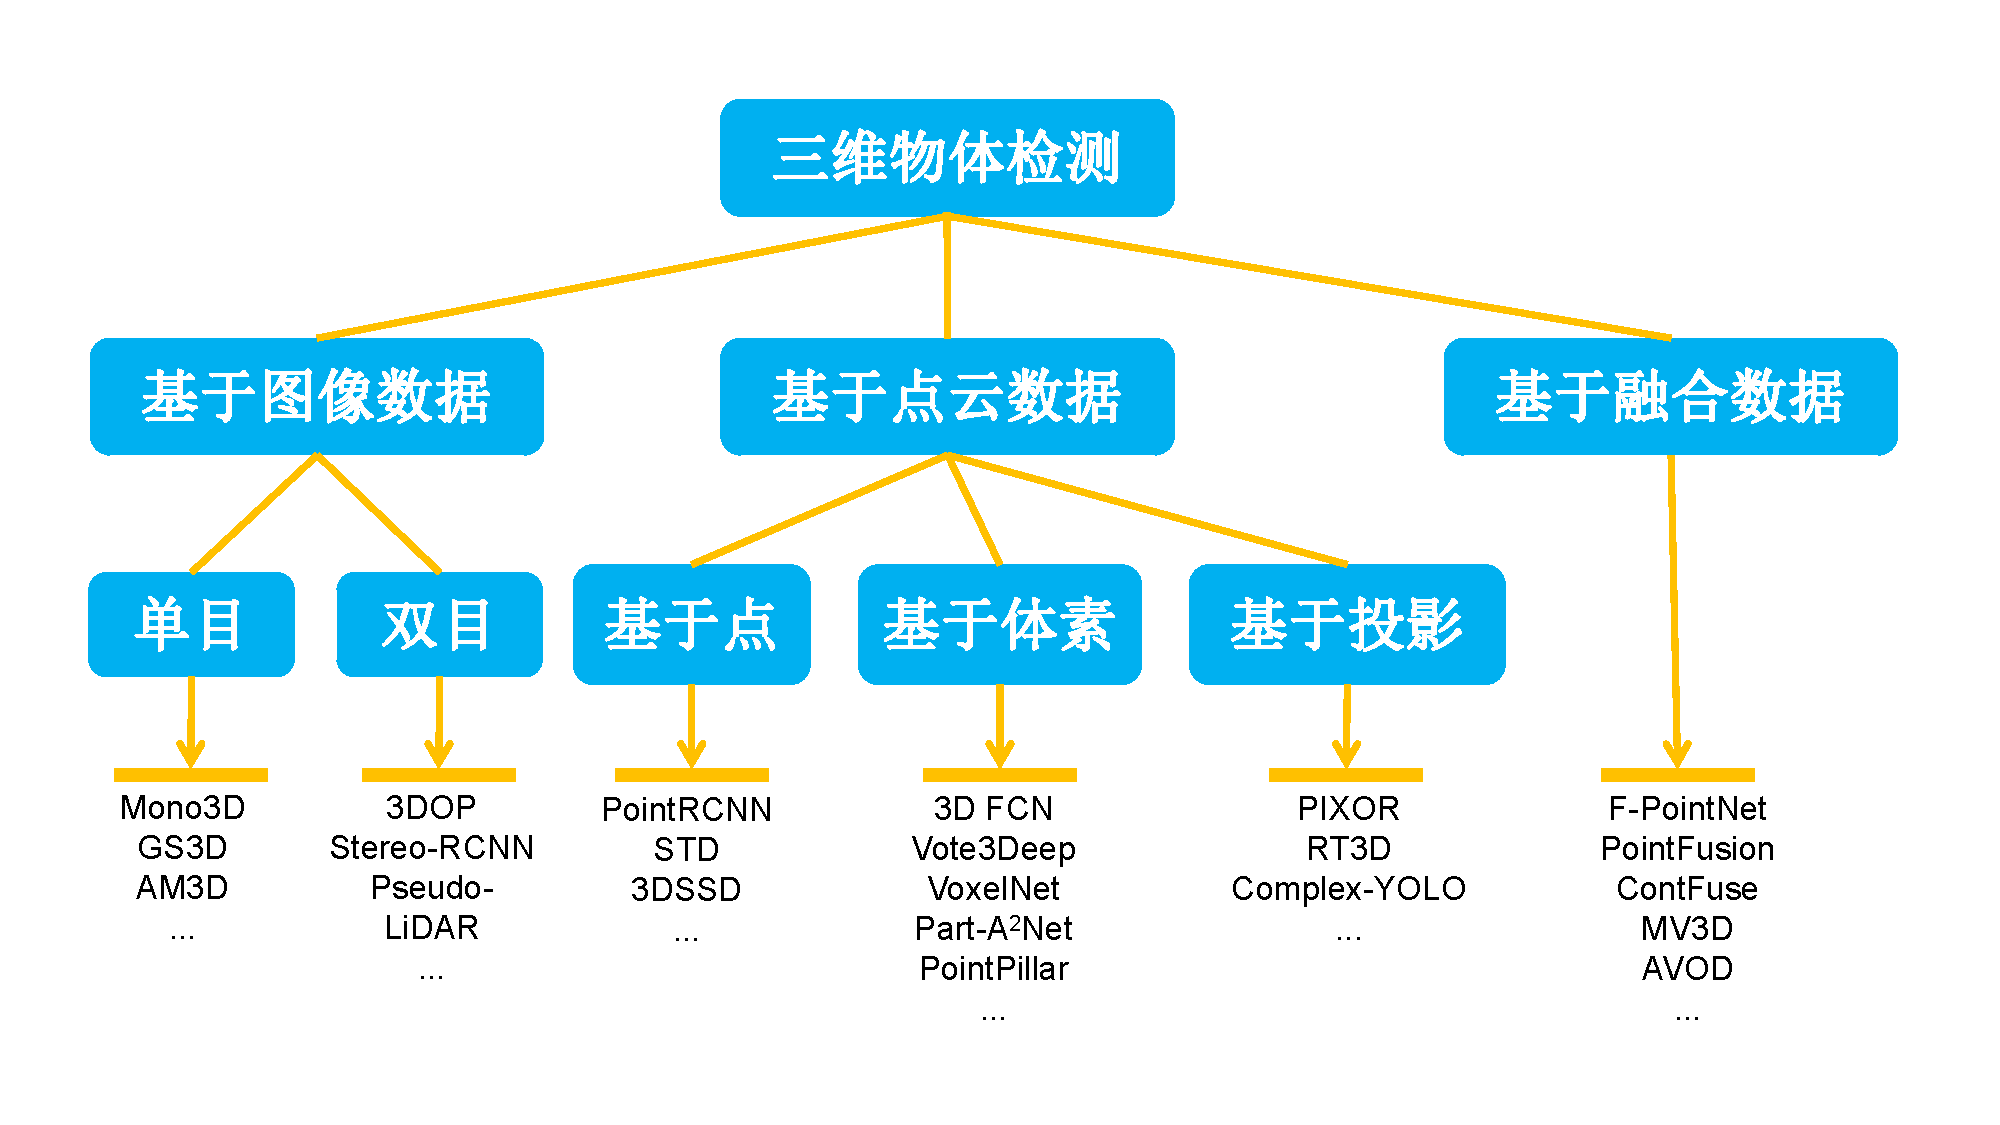
\includegraphics[trim={1.5cm, 1.5cm, 1.5cm, 1.5cm}, clip, width=\textwidth]{imgs/det_algo.pdf}
	\end{center}
	\vspace{-0.8cm}
	\caption{三维物体检测方法分类。}
	\label{fig:det_algo}
\end{figure}


\subsubsection{基于图像数据的三维物体检测}

基于图像数据的三维物体检测有两大类,一类是使用单目摄像头数据,另一类是使用多目(一般为双目)摄像头数据。对于单目摄像头数据,由于摄影几何学的限制,只凭一幅图像是无法恢复出像素点的三维信息的,也无法获得物体的真实的尺寸信息。然而对于特定类型的物体是有可能的,这是因为特定类型的目标往往具有很强的先验信息。这些信息可以被用来构建目标的几何模型,从而使三维物体检测能够顺利进行。对于单目图像三维物体检测,目前有基于目标几何约束提取3D候选框然后将其投影到图像平面提取特征进行预测的,如Mono3D \cite{7780605};也有先对图像进行二维目标检测得到二维边界框,然后利用先验信息对车辆的3D位姿进行建模,从而得到车辆的三维边界框,如\cite{Mousavian3D}以及GS3D\cite{li2019gs3d};另外也有工作使用现有2D物体检测框架以及深度图预测网络得到2D边界框和深度图像,然后再根据相机参数将深度图转换为三维点云,然后利用2D边界框对点云进行分割,最后嵌入RGB信息并使用PointNet\cite{qi2017pointnet}回归出三维边界框,如AM3D\cite{ma2019accurate}。然而,使用单张图像毕竟无法很好地获得物体三维信息,因此这类方法需要人工设计的几何特征来表征物体的深度信息。虽然数据采集简单,速度快,但是检测精度差,落地难。

双目摄像头从生物学上来说很接近人类的双眼视觉系统。对于双目摄像头数据,可以进行双目立体视觉匹配,通过相机之间的相对位置信息可以得到像素点的深度,从而可以在一定程度上恢复物体的三维信息。双目视觉相比于单目视觉有着更强的空间约束关系,因此结合场景先验,可以得到比单目相机更准确的三维物体检测结果。例如,对于两幅成对的图像,3DOP\cite{chen20183d}首先采用了Yamaguchi的方法\cite{Yamaguchi2014Efficient}计算每个像素的深度,生成点云数据,然后采用Struct-SVM\footnote{http://www.cs.cornell.edu/people/tj/svm\_light/svm\_struct.html}优化方法\cite{structSVM}提取3D候选框,最后采用与Fast-RCNN\cite{girshick2015fast}类似框架对3D候选框进行判别和回归,得到最终的预测框。Stereo RCNN\cite{licvpr2019}则将Faster-RCNN\cite{ren2015faster}网络扩展到双目立体视觉,将左右图像输入两个相同的候选框提取网络,然后通过自动对齐学习计算出左右视图中匹配的候选框,最后通过稠密匹配优化得到最终的三维检测结果。此外,还有工作使用双目相机数据生成伪激光雷达数据,然后使用这些点云数据进行三维物体检测。伪激光雷达数据的生成一般使用的是DRON\cite{DRON}或PSMNET\cite{chang2018pyramid}等深度估计网络,这类方法的代表是Pseudo-LiDAR\cite{Wang_2019_CVPR,you2020pseudolidar}。不过双目视觉对于远处的像素点深度估计非常不准,并且存在盲区,因此基于双目视觉的三维物体检测方案存在自身的理论缺陷,只能依靠神经网络根据先验信息弥补系统误差。

\subsubsection{基于点云数据的三维物体检测}

基于点云数据的方案是三维物体检测的主流方向,根据点云数据的特征提取方式不同这些方法又可分为Point-based、Voxel-based 以及Projection-based,本小节将详细介绍这三类方法。

Point-based的方法是直接在点云中提取特征,可以使用PointNet\cite{qi2017pointnet}, PointNet++\cite{qi2017pointnet++}, PointCNN\cite{PointCNN}, PointSIFT\cite{JiangPointSIFT}, Octnet\cite{RieglerOctNet}, Dynamic Graph CNN\cite{WangDynamic}等方法提取点的特征。Point-based的方法中比较有代表性的是香港中文大学提出的PointRCNN\cite{shi2019pointrcnn}以及其后续工作STD\cite{std2019yang}和3DSSD\cite{yang3DSSD20}。PointRCNN方法分为两步,第一步是将整个场景的点云分割为前景点和背景点,然后以自下而上的方式生成高质量候选框;第二步是将每个候选框进行坐标规范化,以便更好的学习局部空间特征然后生成更精确的边界框。STD在此基础上提出了一种基于球形锚点框的点云候选区域提取网络,然后引入了新的点池化层将候选区域内部点的特征从稀疏表达转化为稠密表达。相比于PointRCNN,STD具有更高的召回率以及更少的计算量。3DSSD是同一个研究团队提出的更加轻量型的单阶段三维物体检测网络,该网络提出了一种新的融合采样策略替代之前的上采样层,能够在准确率和速度上达到很好的平衡。这些方法在点云特征提取上都借鉴了PointNet++的思想,特别是使用\textit{set abstraction}操作在点云特征提取中引入可变的感受野。

Voxel-based的方法使用三维体素网格编码点云特征, 每个体素立方体的值由该立方体内的点决定,从而将不规则的三维点云数据编码成规则的三维体素数据, 便于后续使用神经网络进行特征提取。 这方面的代表工作有 3D FCN \cite{li20173d}、Vote3Deep \cite{engelcke2017vote3deep}、 VoxelNet \cite{zhou2018voxelnet}、Part-$A^2$Net\cite{shi2020part}以及PointPillar\cite{lang2018pointpillars}等。3D FCN和Vote3Deep直接对网格化的点云数据使用3D卷积提取特征,由于点云非常稀疏并且3D卷积需要在三个维度上操作,因此整个检测、定位的过程极其耗时。此外,受到感受野的影响,传统的3D CNN并不能很好的学习不同尺度的局部特征。VoxelNet只对非空的网格进行特征提取,并且使用多尺度结构学习不同尺度的信息,一定程度上弥补了这类方法的劣势。Part-$A^2$Net直接引用了VoxelNet的体素化方法,使用了稀疏卷积以及子流型稀疏卷积(Submanifold Sparse Convolution\cite{Graham3D})提取点云特征。PointPillar则是提出新型的垂直柱体网格化方法编码点云特征,使得编码速度更快。这类方法的一大缺点是体素大小不好确定,太大的话信息损失严重,太小则会造成巨大的计算量。 

Projection-based的方法是将点云在高度方向进行投影,将三维数据降维成二维的俯视图(BEV, bird eye view)数据。 考虑到在驾驶场景中, 道路基本是共面且水平的,因此在高度方向上投影对物体的位姿信息基本没有损失。 经过投影操作后,就能直接使用二维图像物体检测的方法进行物体检测。 PIXOR \cite{yang2018pixor}、RT3D\cite{8403277} 以及 Complex-YOLO \cite{simon2018complex,Simon_2019_CVPR_Workshops} 等属于这类方法,这些方法主要不同点在于点云的投影视角以及投影方式。 虽然降维能够带来速度的极大提升,然而由于点云数据的稀疏性,经过投影后目标的特征点损失很严重。 特征点的不足会很大程度上影响检测结果的准确性,特别是对于远处的目标以及小目标。

\subsubsection{基于多传感器数据融合的三维物体检测}

点云的稀疏性以及图像缺少深度信息都限制着相应方法的性能,一个自然而然的想法就是将这两种数据融合, 从而达到更好的检测性能。 基于多传感器融合的方法通过算法融合点云数据以及图像数据,从而提升三维物体检测的准确率。 这类方法的代表有 F-PointNet \cite{qi2018frustum}、PointFusion\cite{XuPointFusion}、ContFuse\cite{Ming2018Deep}以及 MV3D \cite{chen2017multi}、AVOD \cite{ku2018joint}等。 这些方法的区别主要在于数据融合的方式不同, F-PointNet首先使用二维物体检测方法检测出图像中的所有物体,之后对于每个物体,将其反投影回点云中得到一个视锥区域,之后使用PointNet++\cite{qi2017pointnet++}对该区域内的点进行分割,最后进行框回归。该方法通过先在图像中找出目标的大致区域,从而减少了算法在点云空间的搜索空间。然而,该算法的准确率受二维物体检测精度影响很大,在第一步没有检测出的物体,之后没有其他办法弥补。 PointFusion和ContFuse都是先分别在图像与点云数据中使用网络提取特征,然后将这两类特征进行融合并实现三维物体检测。MV3D 则是将二维物体检测中的区域提取网络扩展到三维空间, 提出了三维特征提取网络分别提取点云以及图像特征, 然后通过一个特征融合模块得到多视角融合特征,最后基于融合特征进行三维物体检测。 AVOD 在 MV3D 的基础上改进了特征提取模块, 引入了编码器-解码器结构从而能够得到全分辨率的特征图, 重点提升了小物体的定位精度。 本文工作中的检测模块是在AVOD框架的基础上进行改进的,使其能支持多帧输入,并引入了时序信息处理模块融合连续帧信息。

\subsection{视频流物体检测}
\label{video_detect}
视频流物体检测与单帧物体检测的主要区别在于是否利用了时序信息。 对于视频流物体检测,时序信息是物体的位姿在时间上的连续性的抽象体现。 目前,大多数视频流物体检测方法都是在两个层面利用时序信息,特征提取层面以及最终的框回归层面。 对于特征处理层面, 一般是根据运动信息将前后帧的的特征整合到关键帧,以增加关键帧的物体特征。 这个过程中需要使用到光流信息,即图像中各像素点的运动方向。 代表有 FGFA \cite{zhu2017flow}系列工作。 一般来说光流信息的获取比较困难,这也是限制该方法进一步发展的主要障碍。 对于在框回归层面利用时序信息,主要的工作有 T-CNN \cite{kang2018t, kang2016object} 与 Seq-NMS \cite{han2016seq}等。 T-CNN 使用预先计算的光流信息将关键帧的检测结果传播到临近帧,而 Seq-NMS 则是通过整合连续几帧的高置信度的候选框来提升目标检测中非极大值抑制(Non-Maximum Suppression,NMS)算法的性能。 最近, 也有一些工作试图通过神经网络学习连续帧之间的的时序信息, 从而避免使用高代价的光流数据。 这类方法的代表有 D\&T \cite{feichtenhofer2017detect}。 D\&T 提出了一个双路目标检测网络,可以同时时间视频流的目标检测以及目标追踪。 该网络可以输入多帧数据进行检测, 并且通过互相关操作(Cross-correlation) 来学习相邻帧之间相同物体的对应关系以及偏移。 本文的算法框架在一定程度上也借鉴了 D\&T 的结构, 不过我们在他的基础上进行了很大的改进,使其能够适应三维物体的流数据检测。

\subsection{三维多目标追踪}
\label{tracking}
目前基本上所有的三维多目标追踪方法都是先对流数据的每一帧进行目标检测,然后再将这些检测框关联起来, 这种范式也被称为 \textit{Tracking by Detection} \cite{lenz2015followme}。 三维多目标追踪的工作有很多,比较有代表性的有 FaF \cite{luo2018fast}, 3D-CNN/PMBM \cite{scheidegger2018mono}以及 DSM \cite{frossard2018end}等。 FaF 使用首先将点云流数据结构化成四维张量,然后构建了一个简单的特征提取网络提取特征,最后使用不同的网络头分别预测得到三维目标检测,多目标追踪以及运动方向预测结果。该方法能够整合前 $n$ 帧的检测结果得到精确的物体运动轨迹。 然而该方法计算量巨大, 并且网络参数调节需要有很高的技巧。  3D-CNN/PMBM 首先构建神经网络从单张图像预测物体的三维位姿, 然后将所有帧的检测框送入泊松多重伯努利 (Poisson Multi-Bernoulli Mixture, PMBM) 混合追踪滤波器进行滤波,得到最终的三维多目标追踪结果。 该方法只使用单帧图像进行三维目标检测,效果有限。 DSM 首先使用单帧三维物体检测框架 MV3D \cite{chen2017multi} 对每一帧数据进行物体检测得到三维检测框, 然后通过一个匹配网络(\textit{Matching net})以及得分网络(\textit{Scoring net})关联所有的检测框。 该方法需要对每一帧数据都进行检测, 并且帧与帧之间的时序信息基本上没有被使用,因此不是针对流数据的高效方法。

\section{本文工作及创新点}
\label{subsec:contribution}
本文提出了一个双路物体检测与追踪(\textbf{D}ual-way \textbf{O}bject \textbf{D}etection and \textbf{T}racking, \textbf{DODT})框架, 实现了流数据场景的高效三维物体检测与追踪。 本框架的构建是基于以下几个观察: (1) 点云能够与图像融合从而丰富物体的视觉特征, 这点在 \cite{chen2017multi,ku2018joint}中得到了证实; (2) 除了通过光流数据, 时序信息也能够通过计算相邻帧间的互相关信息,这点通过 D\&T\cite{feichtenhofer2017detect} 也能够得到验证; (3) 特征在连续帧之间的变化是连续的, 我们可以只对关键帧进行检测,然后将结果传播到非关键帧, 这样可以极大的减少计算量。 对于第一点, 本文借用了 AVOD\cite{ku2018joint} 中的数据融合方案,将点云数据提供的 BEV 信息与图像融合。 对于第二点, 本文构建了一个时序模块(Temporal module), 该模块使用互相光操作在 BEV 空间中计算相邻关键帧的时序特征, 然后预测相同物体在不同关键帧中同时出现的概率以及偏移量。 与 \cite{feichtenhofer2017detect,dosovitskiy2015flownet} 不同的是, 本模块的互相关操作是在后候选框层面进行的,不需要全局计算, 这极大地提高了模块的运行效率。 对于最后一点, 我们将 DODT 框架的目标检测模块设计成了双路结构, 这样该模块就能够同时输入两帧相邻关键帧, 以保证后面时序模块的正确运行。 另外, 为了进一步提高框架的效率, 本文还设计了一个共享 RPN (Shared Region Proposal Network, Shared RPN) 模块, 该模块可以生成供两检测分支共同使用的三维候选框。 最后,为了生成所有帧的检测结果, 本文设计了一个基于运动的框插值算法, 该算法利用关键帧的检测结果以及时序模块预测的信息,插值生成非关键帧的检测结果。 同时, 该差值算法还能够将不同帧的候选框关联起来, 得到多目标追踪结果。

本文的贡献及创新点如下:
\begin{itemize}
	\item 本文提出了名为 DODT 的双路网络, 该网络能够同时精确地完成基于流数据的三维物体检测以及多目标追踪任务。
	\item 本文提出了一个时序模块在候选框层面上编码相邻关键帧之间的时序信息, 相比于\cite{feichtenhofer2017detect,dosovitskiy2015flownet}中方法, 该方法更加灵活,也更加高效。
	\item 本文设计了一个共享 RPN 模块, 能够显著提高相邻多帧目标检测中候选框提取的效率。
	\item 本文开发了一个基于运动的框插值算法, 能够有效的将关键帧的预测框传播到非关键帧, 同时也能够将所有框关联起来, 实现多目标追踪。
\end{itemize}


\section{文章组织与结构}
\label{subsec:structure}
本文的主要内容分为五章。 第一章为引言, 介绍项目的研究背景和意义, 国内外的研究进展以及本文工作的简单介绍和创新点; 第二章介绍本工作涉及到的一些技术的基础理论, 分为目标检测与目标追踪两大块; 第三章详细地介绍了本文提出的框架的构造和原理, 是全文的重点内容; 第四章主要是介绍了本项目的实验设计, 结果展示以及实验结果分析, 该部分也是全文的重点内容; 最后一章总结本文的工作, 然后介绍本文工作的不足之处以及后续的实验计划。 


% 打印时插入必要的空白页
\ifprint
	\newpage
	\thispagestyle{empty}
	\mbox{}
	
	% 避免空白页影响页码编号
	\clearpage
	\setcounter{page}{10}
\fi
	\section{深度神经网络}

\frame
{
  	\frametitle{\secname~ }
  	\begin{block}{前馈神经网络}
	  	传统的人工神经网络
  	\end{block}
  	\begin{block}{卷积神经网络}
	  	目前最为流行的,广泛应用于视觉任务的神经网络
  	\end{block}
  	\begin{block}{长短记忆网络}
	  	与卷积网络相比,更适用于处理时序信号
  	\end{block}
}

\subsection*{前馈神经网络结构}
\frame{
	\frametitle{}
    \begin{columns}[onlytextwidth]
		\begin{column}{0.5\textwidth}
			\vspace{-1.5em}
		\begin{itemize}
			\item 有向无环图的结构
			\item 输入层(数据特征)
			\item 隐含层(映射后的特征)
			\item 输出层(预测结果)
			\item 反向传播算法(训练方法)
		\end{itemize}
		\end{column}
		\begin{column}{0.5\textwidth}
		\begin{figure}[h] %structure of LSTM
	\centering
	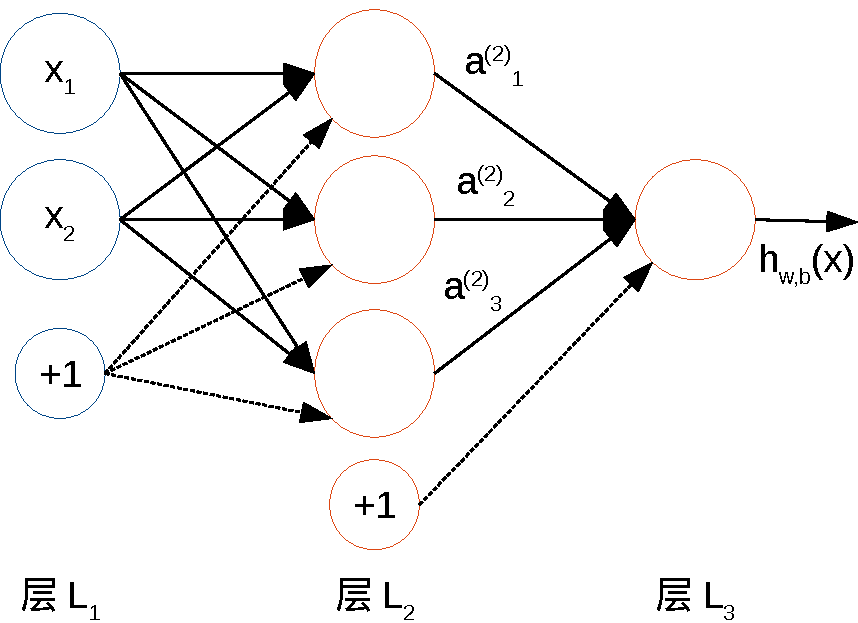
\includegraphics[width=0.9\textwidth]{demo_images/illustration/network1.pdf}
	\caption{前馈神经网络模型示意图}
	\label{fig:lstm}
\end{figure}
		\end{column} 
	\end{columns}
}

\subsection*{卷积神经网络}
\frame{
   	\frametitle{}
   	\vspace{-0.8em}
	\begin{figure}
	\centering
	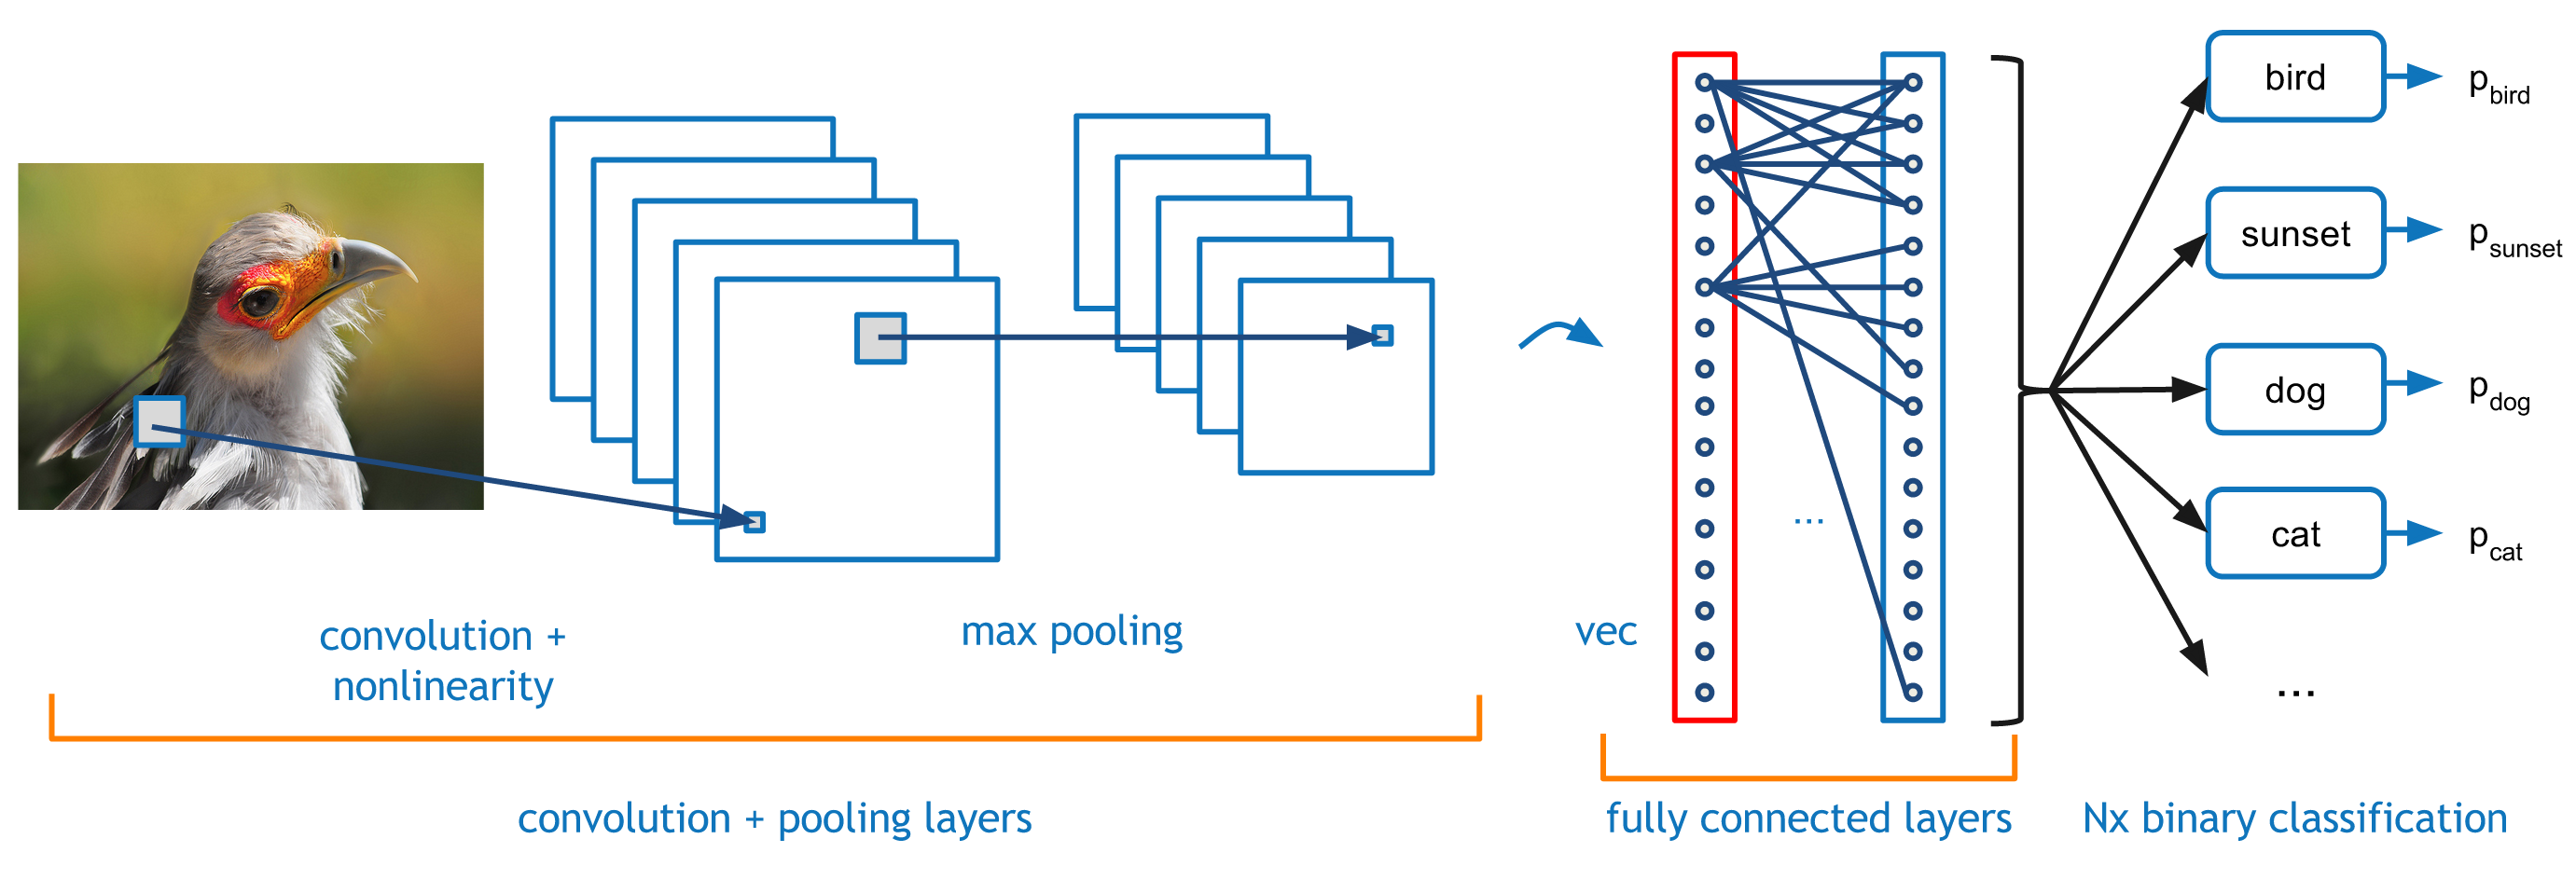
\includegraphics[width=0.8\textwidth]{demo_images/CNN}
	\caption{卷积网络模型示意图}
	\label{fig:network1}
\end{figure}
   	\vspace{-0.8em}
	\begin{block}{与前馈神经网络的区别}
	\begin{itemize}
		\item 直接作用于二维图像,无需特征设计阶段
		\item 卷积层,池化层
		\item 局部感知域,权重共享
	\end{itemize}
	\end{block}
}

\subsection*{长短记忆网络(处理一维信号)}
\frame{
	\frametitle{}
	\tiny
	\vspace{-2em}
    \begin{columns}[onlytextwidth]
        \begin{column}{0.5\textwidth}
	    \begin{figure}[h] %structure of LSTM
   	\centering
   	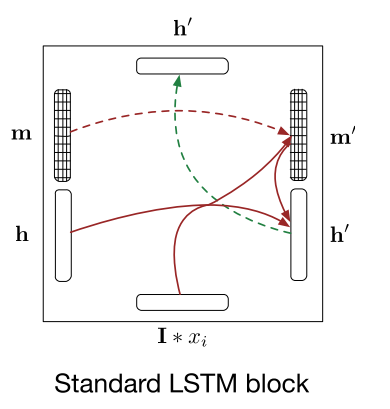
\includegraphics[width=0.6\textwidth]{demo_images/lstmblock1}
   	\caption{长短记忆网络区块示意图}
   	\label{fig:lstm}
\end{figure}
		\end{column} 
		%%%%%%% new column
		\begin{column}{0.5\textwidth}
			\begin{boxedminipage}{0.8\textwidth}
			\vspace{-1.5em}
			\begin{align}
				\label{eq:lstm}
				\begin{split}
				\textbf{g}^u &= \delta(\textbf{W}^u*\textbf{H}) \\
				\textbf{g}^f &= \delta(\textbf{W}^f*\textbf{H}) \\
				\textbf{g}^o &= \delta(\textbf{W}^o*\textbf{H}) \\
				\textbf{g}^c &= \mbox{tanh}(\textbf{W}^c*\textbf{H}) \\
				\textbf{m}' &= \textbf{g}^f \odot \textbf{m} + \textbf{g}^u \odot \textbf{g}^c \\
				\textbf{h}' &= \mbox{tanh}(\bf{g}^o \odot \bf{m}') \\
					\textbf{H} & = \begin{bmatrix}
					I*\textbf{x}_i \\ \textbf{h}
					\end{bmatrix}
			\end{split}
			\end{align}
		\end{boxedminipage}
		\end{column}
    \end{columns}
	
	\vspace{-1em}
	\begin{block}{缩写形式}
	\footnotesize
	\begin{equation*}
		(\textbf{h}', \textbf{m}') = \mbox{LSTM}\bigr(\textbf{H},\textbf{m},\textbf{W} \bigr)
	\end{equation*}
	其中\textbf{W}包含了四个门权值矩阵$\textbf{W}^u,\textbf{W}^f,\textbf{W}^o,\textbf{W}^c$。
	\end{block}
}

\subsection*{网格型长短记忆网络(处理N维信号)}
\frame{
	\frametitle{}
	\vspace{-1.5em}
	\begin{figure}[h]
	\centering
	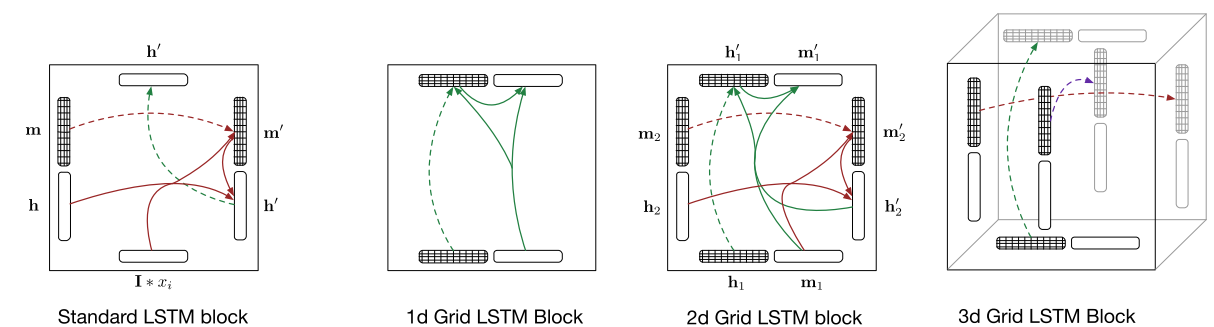
\includegraphics[width=\textwidth]{demo_images/gridlstm}
	\caption{网格型长短记忆网络区块示意图[Kalchbrenner et al, Grid LSTM, ICLR 2016]}
\end{figure}
	\vspace{-2em}
	\begin{block}{网格型长短记忆网络更新过程}
	\tiny
	\begin{columns}[onlytextwidth]
		\begin{column}{0.4\textwidth}
		\vspace{-0.5em}
			\begin{equation}
				\textbf{H} = \begin{bmatrix}
					\textbf{h}_i \\ \vdots \\ \textbf{h}_N
				\end{bmatrix}
			\end{equation}
		\end{column}
		\begin{column}{0.6\textwidth}
		\vspace{-1em}
			\begin{align}
				\begin{split}
				(\textbf{h}_1', \textbf{m}_1') & =  \mbox{LSTM}(\textbf{H}, \textbf{m}_1, \textbf{W}_1) \\ &\mbox{ }\vdots \\
				(\textbf{h}_N', \textbf{m}_N') & =  \mbox{LSTM}(\textbf{H}, \textbf{m}_N, \textbf{W}_N)
				\end{split}
				\label{eq:gridlstm}
			\end{align}
		\end{column}
	\end{columns}
	\end{block}
}
\endinput

	\section{网络模型结构}

\subsection*{网络整体结构}
\frame{
	\begin{figure}[h]
	\centering
	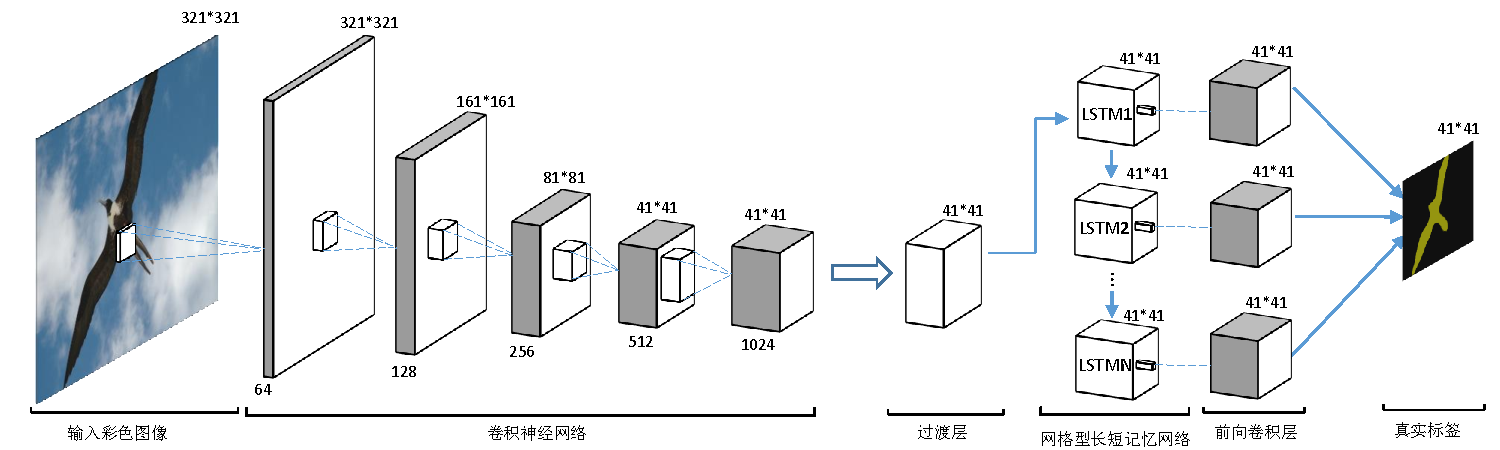
\includegraphics[width=0.9\textwidth,height=0.28\textwidth]{demo_images/illustration/networkstructure.pdf}
	\caption{网络整体结构图}
	\label{fig:networkstructure}
\end{figure}
	\vspace{-1em}
	\small
	\begin{block}{}
	\begin{itemize}
		\item  四个组成部分:\textbf{卷积网络部分},过渡层,\textbf{网格型长短记忆网络部分},前向卷积层
		\item 核心思想:在卷积网络后堆叠多层网格型长短记忆层
	\end{itemize}
	\end{block}
}

\subsection*{卷积网络部分}
\frame{
	\frametitle{}
	\vspace{-1em}
	\footnotesize
	\begin{block}{}
	\begin{itemize}
		\item 基于$VGG_{16}$模型\footnote{Simonyan \& Zissermanet, Very deep Convolutional Networks For Large-scale Image Recognition, ICLR 2015}, 含有16层卷积层
		\item 使用了“孔算法”,在不损失精度的情况下将模型参数减少了 6.5 倍\footnote{Chen et al, DeepLab-LargeFOV, ICLR 2015}
	\end{itemize}
	\end{block}
	\vspace{-1em}
	\begin{figure}[h]
	\centering
	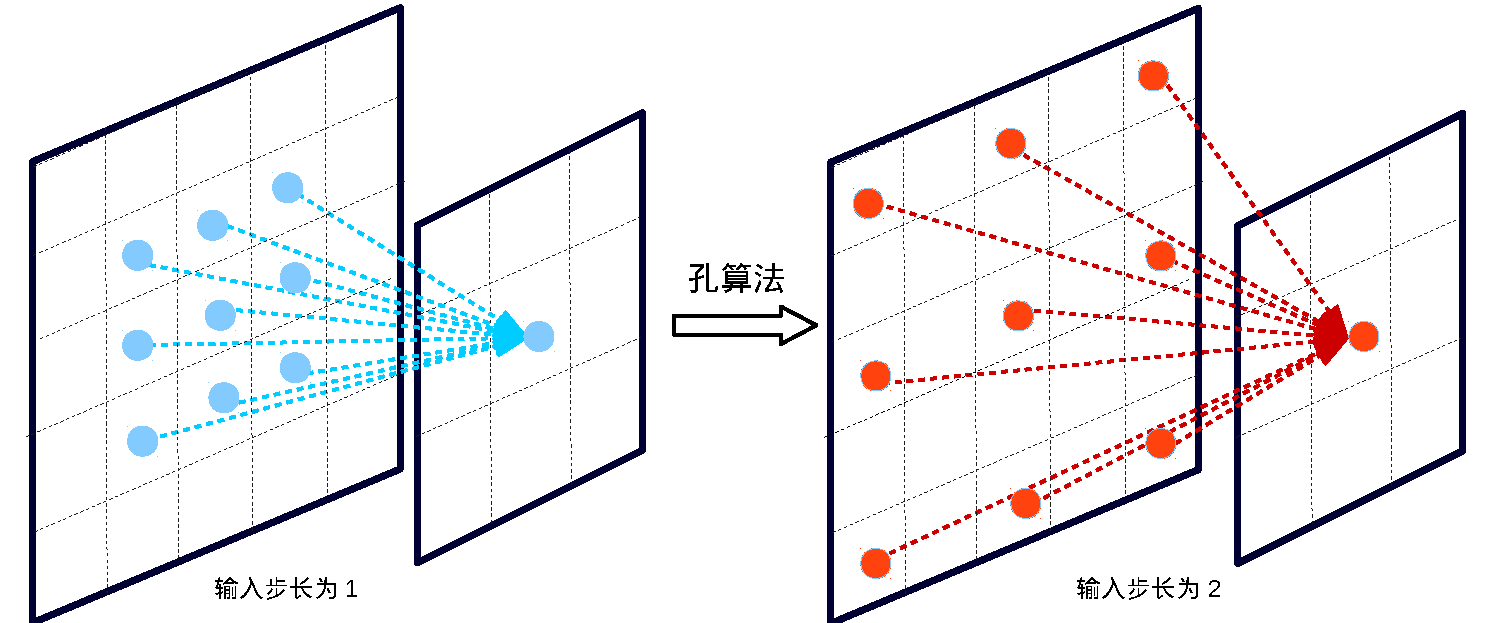
\includegraphics[width=0.7\textwidth]{demo_images/illustration/hole.pdf}
	\caption{"孔算法"示意图}
\end{figure}
}


\subsection*{网格型长短记忆网络部分}
\frame{
	\frametitle{}
	\vspace{-1em}
    \begin{columns}%[onlytextwidth]
        \begin{column}{0.6\textwidth}
        \vspace{0.2em}
		\begin{figure}
	\centering
	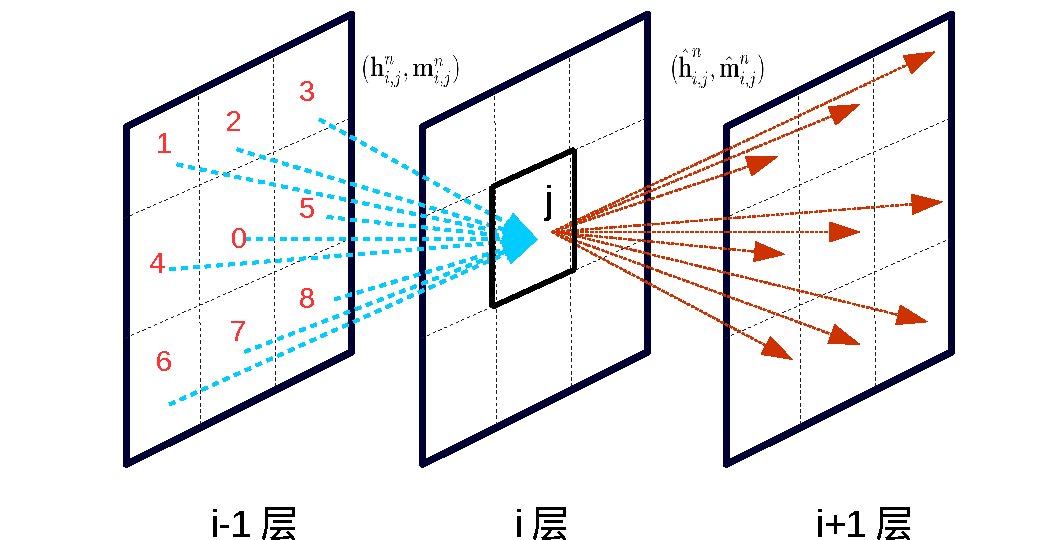
\includegraphics[width=\textwidth]{demo_images/illustration/neighboring.pdf}
	\caption{九维网格型长短记忆网络层之间的通信示意图}
	\label{fig:neighboring}
\end{figure}
		\end{column} 
		%%%%%%% new column
		\begin{column}{0.5\textwidth}
			\footnotesize
			\vspace{-1.5em}
			\begin{align}
				\begin{split}
				(\hat{\textbf{h}}_{i,j}^0,\hat{\textbf{m}}_{i,j}^0) &= \mbox{LSTM}(\textbf{H}_{i,j},\textbf{m}_{i,j}^0,\textbf{W}_i) \\
				(\hat{\textbf{h}}_{i,j}^1,\hat{\textbf{m}}_{i,j}^1) &= \mbox{LSTM}(\textbf{H}_{i,j},\textbf{m}_{i,j}^1,\textbf{W}_i) \\
				\vdots \\
				(\hat{\textbf{h}}_{i,j}^N,\hat{\textbf{m}}_{i,j}^N) &= \mbox{LSTM}(\textbf{H}_{i,j},\textbf{m}_{i,j}^N,\textbf{W}_i) \\
				\textbf{H}_{i,j} &= [\textbf{h}_{i,j}^0\mbox{ }\textbf{h}_{i,j}^1\mbox{ }...\mbox{ }\textbf{h}_{i,j}^N]^T
				\end{split}
			\end{align}
		\end{column}
    \end{columns}
	\footnotesize
	\vspace{-1em}
	\begin{block}{九维网格型长短记忆网络}
		\vspace{-0.7em}
		\begin{itemize}
			\item 每个位置的预测会受到上一层相邻八邻域特征的影响
			\item 随着层数的堆叠,每一位置将会有更大的感知域。
			\item 网格型长短记忆网络的层数通过实验来确定
		\end{itemize}
	\end{block}
}
	% !Mode:: "TeX:UTF-8"

\chapter{实验过程与结果分析}
\label{experiment}
本章将介绍本项目的实验部分,包括对KITTI数据集、数据预处理、模型训练以及实验结果分析等内容。在结果分析中,我们首先比较DODT各模块对结果的影响,以考察每个模块的有效性;然后我们探讨了关键帧的选取步长对三维物体检测结果的影响,以便确定最优的步长;最后我们也测试了DODT在多目标追踪任务上的性能,并与前沿方法对比。结果显示DODT框架能很好的完成流数据的三维物体检测以及多目标跟踪任务。

\section{KITTI数据集介绍}
\label{kitti}
本项目的所有实验都是基于无人驾驶领域中广泛使用的KITTI公开数据集开展的。KITTI数据集是由德国卡尔斯鲁厄理工学院和丰田美国技术研究院联合采集的,该数据集包含多种传感器数据:一个惯性导航系统(GPS/IMU,型号为OXTS RT 3003)数据,一个激光雷达(Velodyne HDL-64E)数据,两个灰度相机数据(140万像素)以及两个彩色相机数据(140万像素)。其中激光雷达扫描频率为10帧/秒,相机基本与地平面保持平行,图像采集的尺寸为$1382 \times 512$像素。所有传感器的整体布局如\figurename \ref{fig:KITTI}。

\begin{figure}[h]
	\centering
	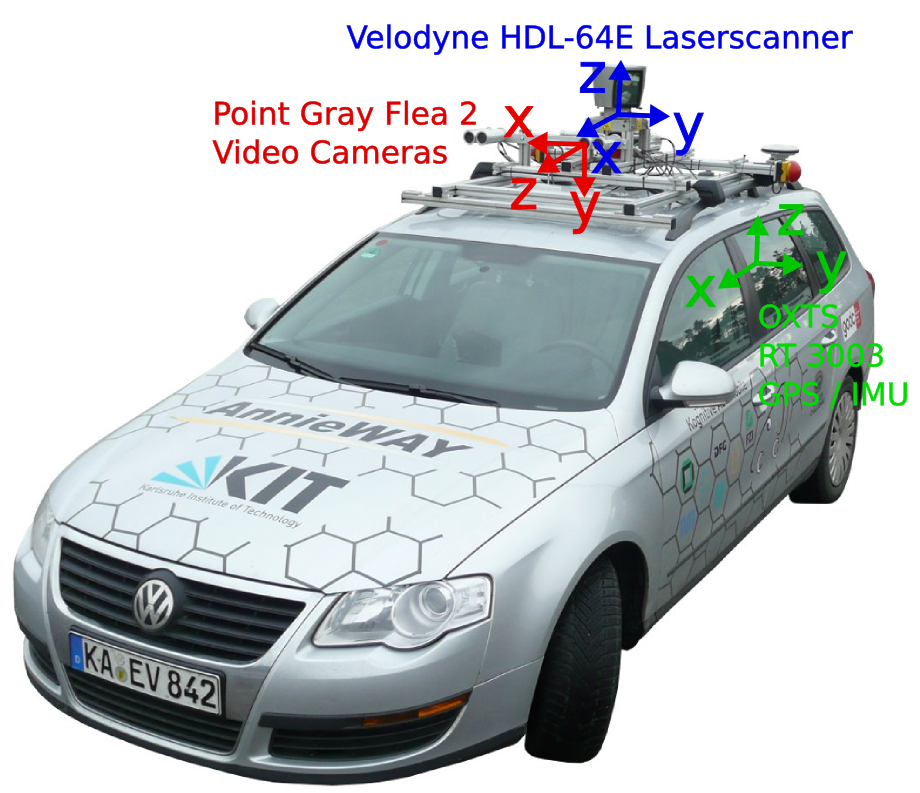
\includegraphics[width=0.6\textwidth]{./imgs/KITTI.png}
	\caption{KITTI数据集传感器整体布局。}
	\label{fig:KITTI}
\end{figure}

KITTI数据集根据不同的任务分为stero、flow、scenceflow、depth、odometry、object以及tracking等部分,对应着场景流估计、深度估计、路径规划、物体检测以及目标追踪等任务。每一个任务数据包都包含了海量的训练数据以及测试数据,供研究者使用。本项目主要使用了KITTI数据集的tracking数据包,该数据包由21段训练视频流(共8004帧数据)以及29段测试视频流(共11095帧数据)组成。每一段视频流都是由连续的RGB图像帧以及三维点云帧组成,在训练数据集中,还包含了每一帧数据对应的二维目标框(针对图像数据)以及三维目标框(针对点云数据)。此外,针对每一段视频流,KITTI还提供了传感器的标定信息以及每一帧的GPS/IMU数据,供研究者数据标定时使用。

多目标追踪的标签共有10项,记录了帧的信息以及帧中每个目标的信息。信息列举如下:
\begin{itemize}
	\item frame id:帧的编号;
	\item object id:每一帧中目标的编号,也是轨迹的编号;
	\item type:目标的类别,有”Car“,”Van“, "Trunk",”Pedestrian“,”Cyclist“等类别,本实验将”Car“和”Van“合并为”Car“类,并只针对”Car“类进行检测和追踪;
	\item truncated:标记目标是否被图像边界截断,”0“表示不截断,”1“表示截断;
	\item occluded:标记目标被遮挡的程度,共有0到3四个取值,”0“表示完全可视,”1“表示部分遮挡,”2“表示大部分遮挡,”3“表示完全遮挡;
	\item alpha:目标的观测角,$\alpha \in [-\pi, \pi]$;
	\item bbox:物体在图像上的2D边界框,包含左上角,右下角的坐标值;
	\item dimensions:物体的高、框和长,单位为米;
	\item location:物体底部中心点在相机坐标系的三维坐标 x,y,z,单位为米;
	\item ry:物体在相机坐标系沿Y轴的旋转角,$r_y \in [-pi, pi]$。
\end{itemize}
其中目标的观测角$\alpha = -[(\pi+r_y) + (\pi+\beta)]$,$r_y$与$\beta$如\figurename \ref{fig:kitti_obj}所示,而目标的location坐标如\figurename \ref{fig:kitti_box3d}所示。
\begin{figure}[!t]
	\centering
	\begin{minipage}[t]{0.5\textwidth}
		\centering
		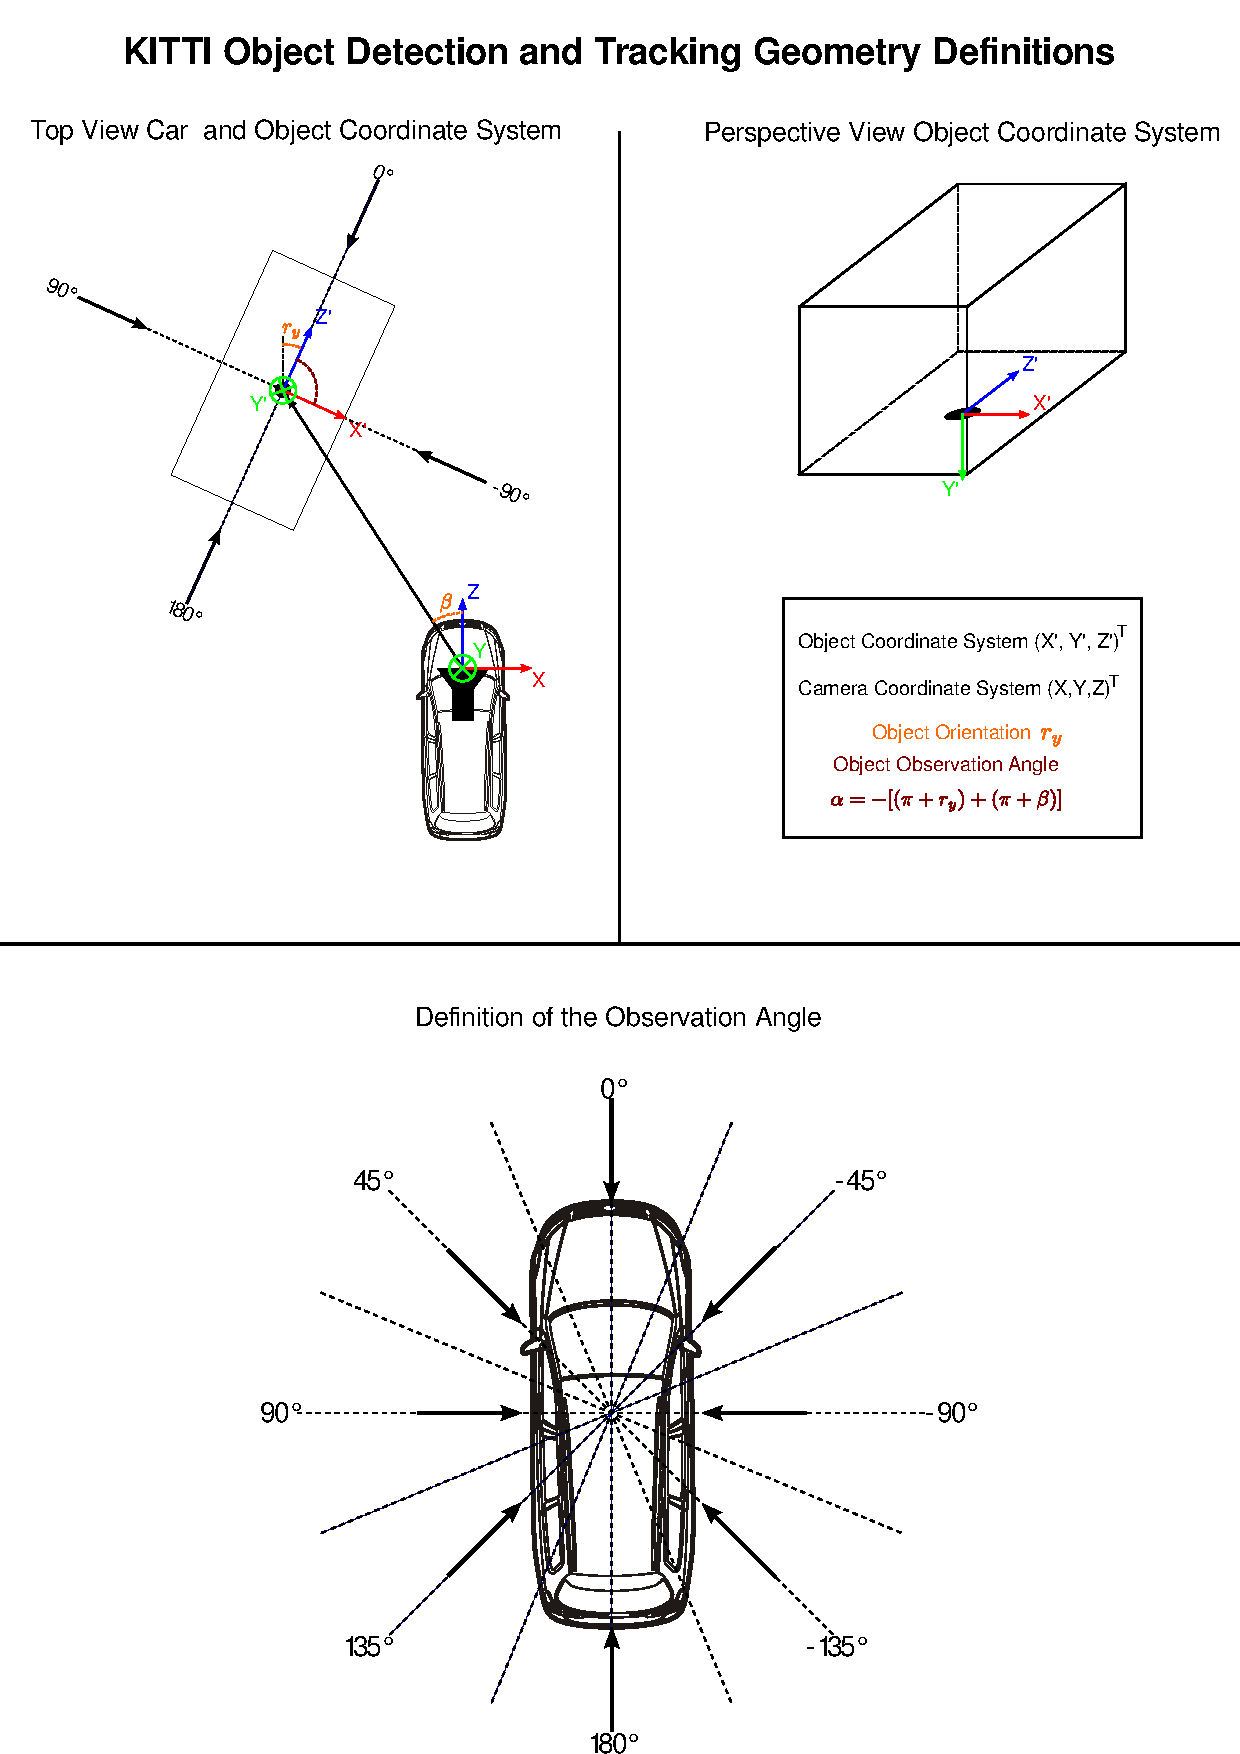
\includegraphics[trim={0cm, 15cm, 12cm, 2.5cm}, clip,width=\textwidth]{./imgs/KITTI_obj.pdf}
		\caption{KITTI数据集观测角与转向角示意图。}
		\label{fig:kitti_obj}
	\end{minipage}
	\begin{minipage}[t]{0.48\textwidth}
		\centering
		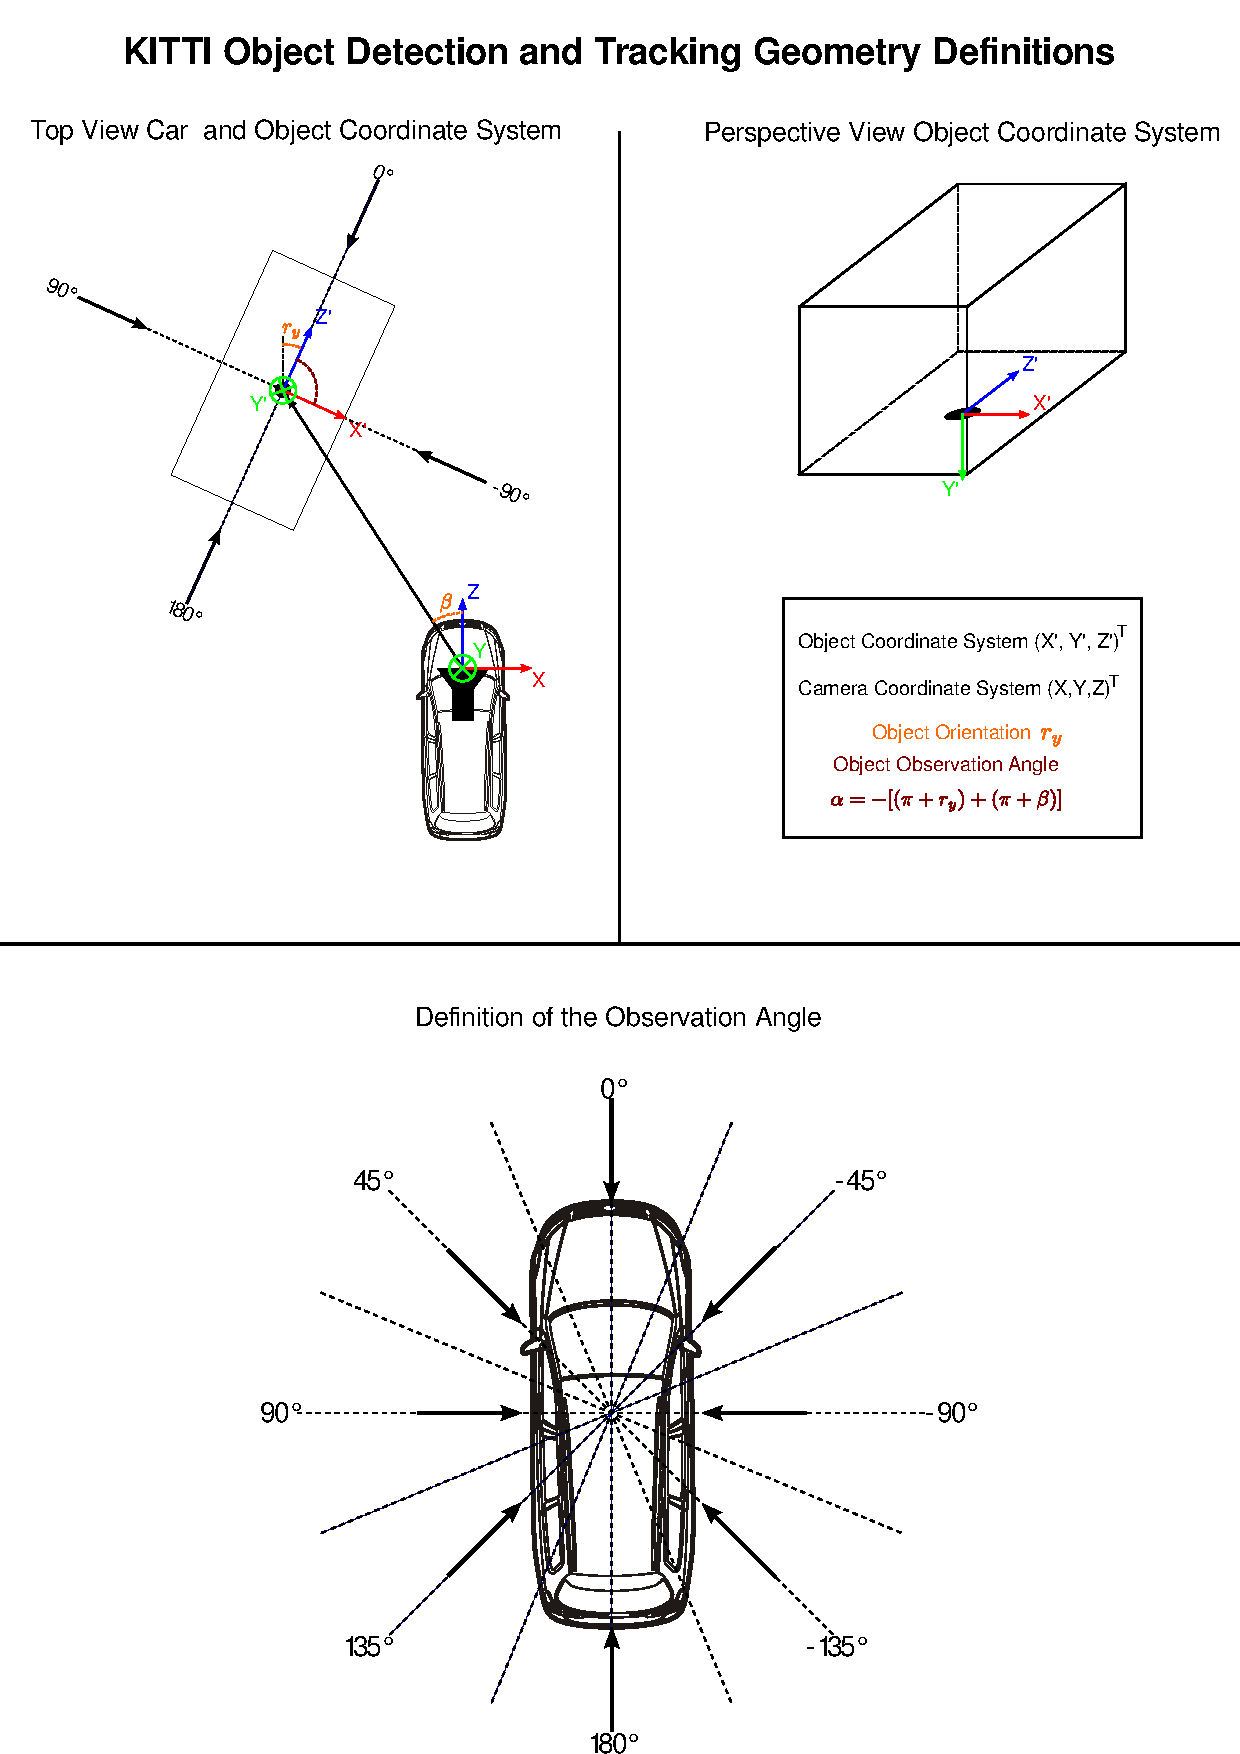
\includegraphics[trim={12cm, 20cm, 1.8cm, 2.5cm}, clip,width=\textwidth]{./imgs/KITTI_obj.pdf}
		\caption{KITTI数据集目标的位置坐标。}
		\label{fig:kitti_box3d}
	\end{minipage}
\end{figure}


传感器的标定信息保存在”calib.txt“文件中,其中包含了相机的参数矩阵以及各传感器之间的旋转矩阵。信息列举如下:
\begin{itemize}
	\item P0-P3:四个相机的内参矩阵 $P \in \mathcal{R}^{3\times 4}$;
	\item R0\_rect:$\mathcal{R}^{3\times 3}$,将摄像机坐标系转换到图像坐标系的校准矩阵;
	\item Tr\_velo\_to\_cam:$\mathcal{R}^{3\times 4}$,激光雷达坐标系到摄像机坐标系的旋转矩阵;
	\item Tr\_imu\_to\_velo:$\mathcal{R}^{3\times 4}$,IMU坐标系到激光雷达坐标系的旋转矩阵。
\end{itemize}

GPS/IMU数据提供了30项信息,其中包含每一帧中自身车辆的经纬度、海拔、三个欧拉角(roll,yaw以及pitch)、速度、加速度、角速度等信息。本实验主要使用到了经纬度以及欧拉角信息将不同帧之间的信息校准到同一坐标系。欧拉角包含了偏航角(yaw,表示机体轴在水平面上的投影与地轴之间的夹角,右偏为正)、俯仰角(pitch,表示机体轴与地平面之间的夹角,抬头为正) 以及翻滚角(roll,表示机体对称面绕机轴转动的角度,右滚为正),如\figurename \ref{fig:euler}所示。
\begin{figure}[t]
	\centering
	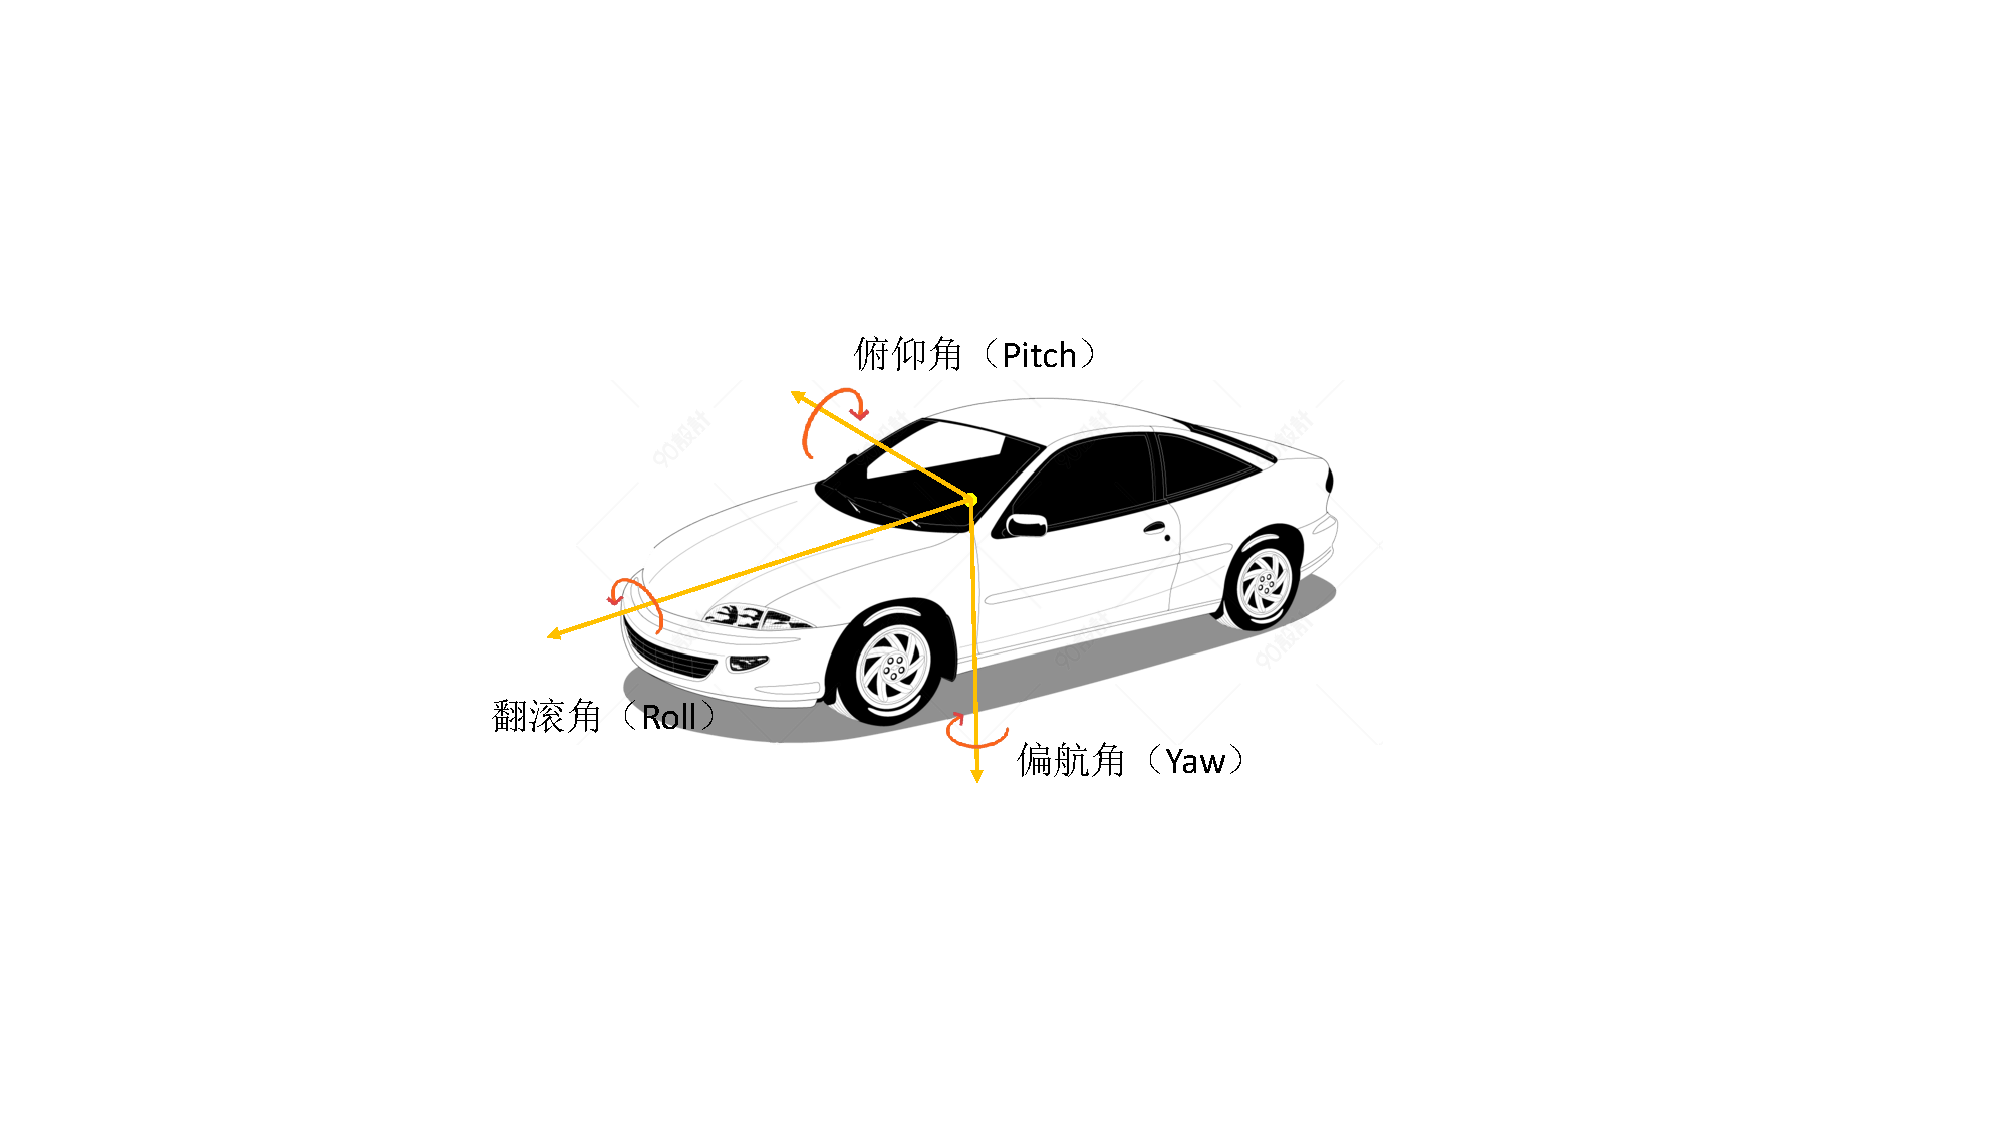
\includegraphics[trim={5cm, 6cm, 5cm, 5cm}, clip,width=\textwidth]{./imgs/euler.pdf}
	\caption{三个欧拉角的方向示意图。}
	\label{fig:euler}
\end{figure}



\section{数据预处理}
\label{preprocessing}


\section{模型训练}
\label{training}


\section{实验结果分析}
\label{results}


\subsection{三维物体检测结果分析}
\label{ablation_study}

\begin{table}[t]
	\centering
	\wuhao
	\caption{候选框预测性能比较。}
	\vspace{0.3cm}
	\begin{tabular}{ccc}
		\toprule[1.5pt]
		方法        & 原始 RPN & \textit{Shared RPN}  \\ \midrule
		准确率(\%)  & 97.81      & \textbf{98.47}       \\
		\bottomrule[1.5pt]
	\end{tabular}
	\label{table:rpn_result}
\end{table}


\begin{table}\centering
	\wuhao
	\caption{DODT的不同设置在验证数据集上的结果(只预测“Car”类别)。每项的指标为$AP_{3D}/AP_{BEV}$ (\%), 为三维物体检测在3D视角和BEV视角的平均精度。 “S” 表示\textit{Shared RPN}模块, “T” 表示时序信息处理模块, “M” 表示运动插值模块。 $\tau$ 是关键帧选取步长。} 
	\vspace{0.3cm}
	\resizebox{\textwidth}{!}{
		\begin{tabular}{ccccccccc}
			\toprule[1.5pt]
			&\multicolumn{1}{c|}{}   & \multicolumn{3}{c|}{IoU = 0.5}  		         & \multicolumn{3}{c|}{IoU = 0.7}          &  \\ \midrule
			\multicolumn{1}{c|}{方法} & \multicolumn{1}{c|}{模块}    & Easy     & Moderate   & \multicolumn{1}{c|}{Hard}     & Easy  & Moderate & \multicolumn{1}{c|}{Hard}    & FPS \\\midrule
			\multicolumn{1}{c|}{AVOD\cite{ku2018joint}}     &\multicolumn{1}{c|}{-}     & 90.13 / 90.91  & 80.00 / 81.79 & \multicolumn{1}{c|}{71.61 / 81.79}  & 76.00 / 90.90 & 57.23 / 81.73 & \multicolumn{1}{c|}{56.13 / 72.69}   & 10.0\\
			\multicolumn{1}{c|}{DODT($\tau$ = 1)}     &\multicolumn{1}{c|}{S}     & 88.28 / 99.97  & 85.74 / 90.90 & \multicolumn{1}{c|}{86.14 / 90.89}  & 83.44 / 90.82 & 67.48 / 90.79 & \multicolumn{1}{c|}{61.24 / 90.80}     & 6.7 \\
			\multicolumn{1}{c|}{DODT($\tau$ = 1)}     &\multicolumn{1}{c|}{S+T}     & 88.32 / \textbf{99.99}  & 86.53 / 90.90 & \multicolumn{1}{c|}{86.71 / \textbf{90.90}}  & 83.60 / 90.82 & 68.93 / 90.80 & \multicolumn{1}{c|}{62.69 / 90.81}   & 5.9\\
			\multicolumn{1}{c|}{DODT($\tau$ = 1)}     &\multicolumn{1}{c|}{S+M}     & 89.99 / 99.95  & 87.86 / 90.87 & \multicolumn{1}{c|}{87.81 / 90.86}  & 86.89 / 90.89 & 73.96 / 90.83 & \multicolumn{1}{c|}{67.07 / 81.79}   & 6.5\\
			\multicolumn{1}{c|}{DODT($\tau$ = 1)}     &\multicolumn{1}{c|}{S+T+M} & \textbf{90.63} / 99.95  & 89.07 / 90.90 & \multicolumn{1}{c|}{88.79 / \textbf{90.90}}  & 88.74 / 90.91 & 75.27 / 90.84 & \multicolumn{1}{c|}{68.75 / 90.57}   & 5.7\\ \midrule
			\multicolumn{1}{c|}{DODT($\tau$ = 2)}     &\multicolumn{1}{c|}{S+T+M} & 90.60 / 99.94  & \textbf{89.19 / 90.91} & \multicolumn{1}{c|}{\textbf{88.91} / 90.88}  & \textbf{88.90 / 90.92} & \textbf{76.64} / 90.85 & \multicolumn{1}{c|}{75.81 / 90.83}   & 8.6\\
			\multicolumn{1}{c|}{DODT($\tau$ = 3)}     &\multicolumn{1}{c|}{S+T+M} & 90.61 / 99.98  & 89.01 / 90.89 & \multicolumn{1}{c|}{88.84 / 90.89}  & 88.81 / 90.91 & 76.38 / \textbf{90.86} & \multicolumn{1}{c|}{\textbf{75.83 / 90.85}}   & 11.4\\
			\multicolumn{1}{c|}{DODT($\tau$ = 4)}     &\multicolumn{1}{c|}{S+T+M} & 90.55 / 99.94  & 88.82 / 90.88 & \multicolumn{1}{c|}{88.34 / 90.87}  & 88.43 / 90.91 & 75.70 / 90.82 & \multicolumn{1}{c|}{68.75 / 90.82}   & 14.3\\
			\multicolumn{1}{c|}{DODT($\tau$ = 5)}     &\multicolumn{1}{c|}{S+T+M} & 87.98 / 90.91  & 85.57 / 90.87 & \multicolumn{1}{c|}{86.01 / 90.87}  & 81.59 / 90.81 & 67.30 / 90.76 & \multicolumn{1}{c|}{61.35 / 81.73}   & 17.1\\
			\multicolumn{1}{c|}{DODT($\tau$ = 6)}     &\multicolumn{1}{c|}{S+T+M} & 78.77 / 90.75  & 70.88 / 90.71 & \multicolumn{1}{c|}{71.65 / 81.70}  & 71.71 / 90.44 & 55.86 / 81.50 & \multicolumn{1}{c|}{56.80 / 81.51}   & \textbf{20.0} \\ 
			\bottomrule[1.5pt]
	\end{tabular}}
	\label{table:result_detection}
\end{table}




\subsection{流数据检测结果分析}
\label{stream_result}

\begin{figure}[!t]
	\centering
	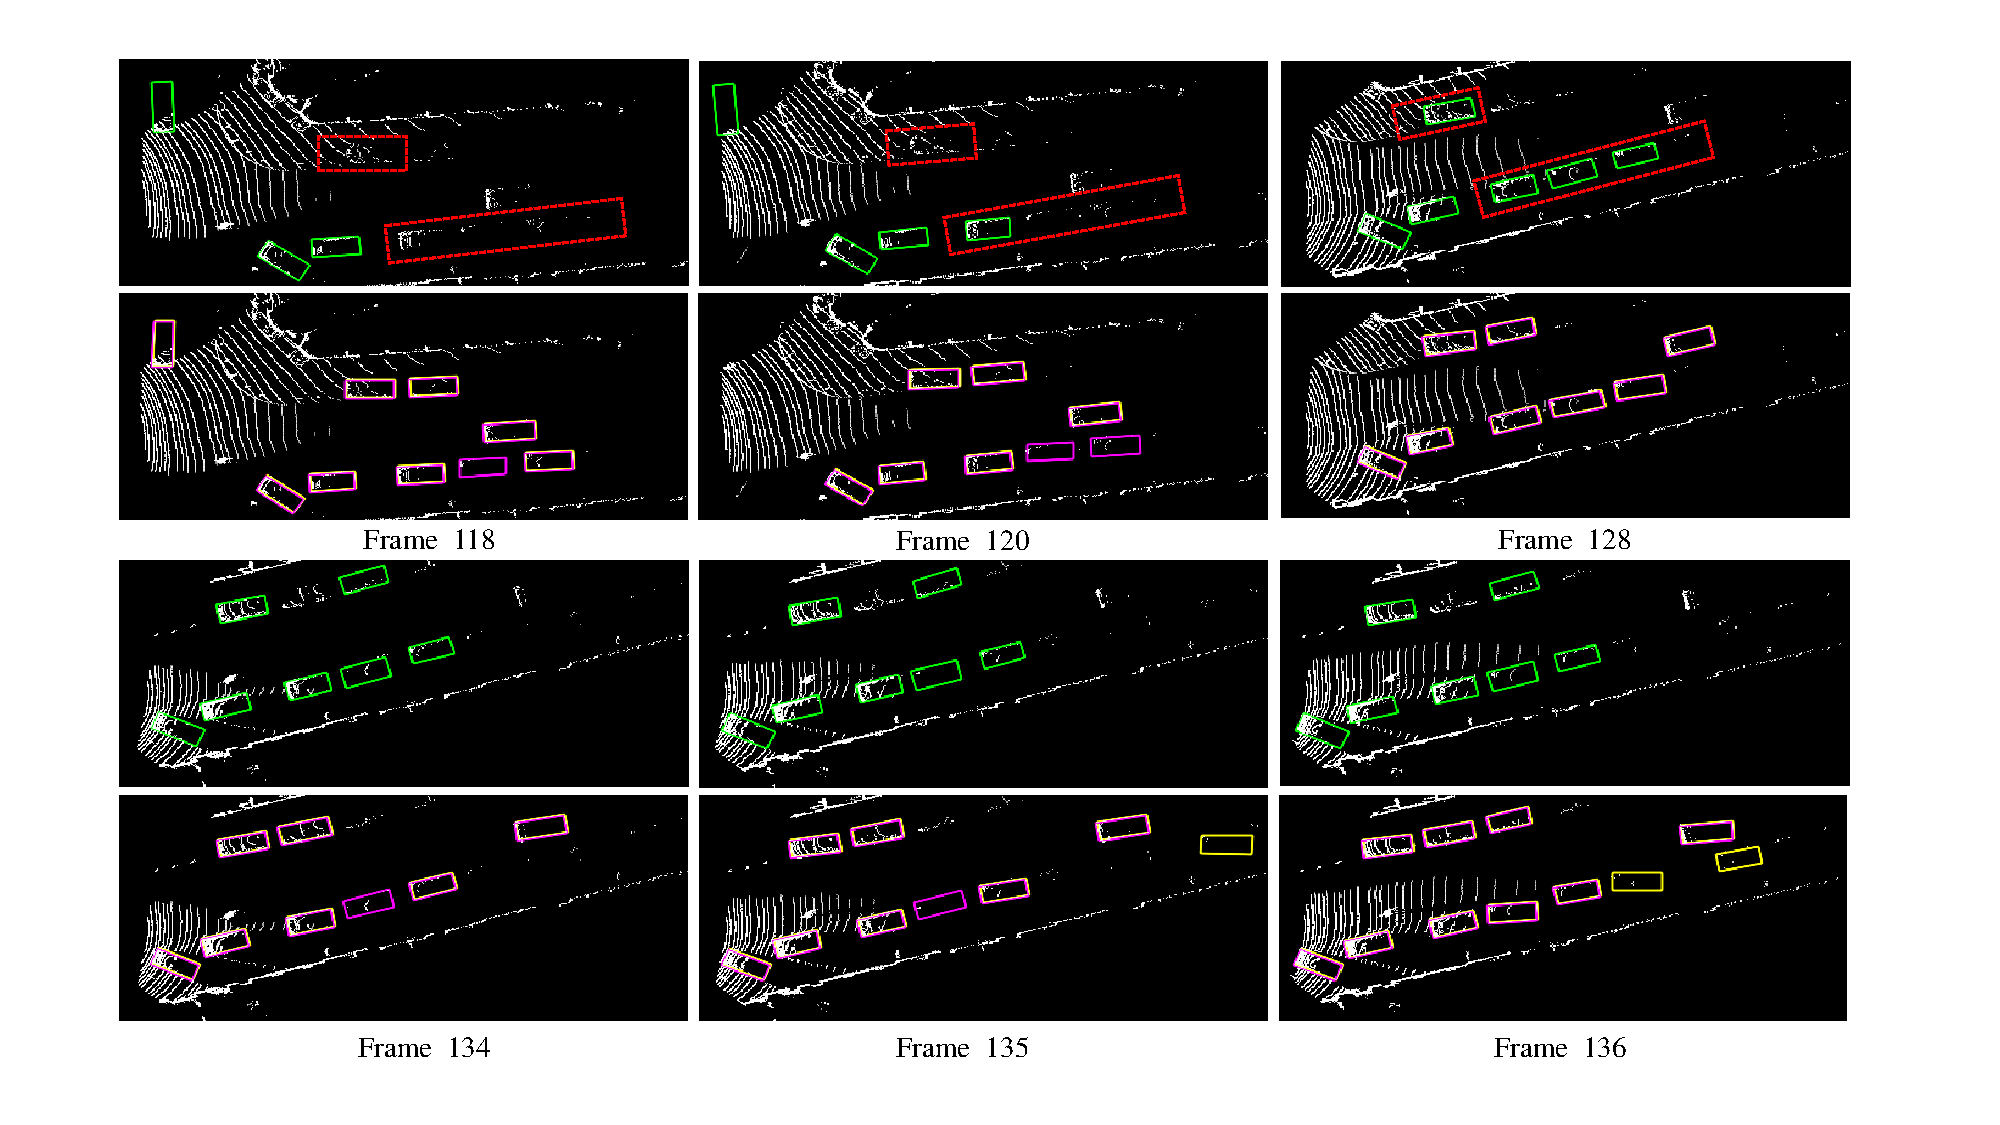
\includegraphics[trim={2cm, 1cm, 2.5cm, 1cm}, clip, width=\textwidth]{./imgs/examples.pdf}
	\vspace{-1.0cm}
	\caption{视频序列0的标签以及预测结果可视化。\textcolor{green}{绿色}为官方提供的标签框, \textcolor{yellow}{黄色}是时序步长$\tau = 1$的预测结果,\textcolor{magenta}{洋红色}为时序步长$\tau = 3$的预测结果。混合颜色的框是黄色框和洋红色框重叠造成的,该结果最好彩色打印查看。}
	\label{fig:examples}
\end{figure}


\subsection{多目标跟踪实验分析}
\label{mot_result}

\begin{table}
	\centering
	\wuhao
	\caption{DODT的不同设置在KITTI多目标追踪验证数据集上的结果。S 表示\textit{Shared RPN}模块, T 表示时序信息处理模块, M 表示运动插值模块。 $\tau$ 是关键帧选取时间步长。}
	\vspace{0.3cm}
	\resizebox{\textwidth}{!}{
		\begin{tabular}{cccccccc}
			\toprule[1.5pt]
			方法   & 模块 & MOTA(\%)$\uparrow$ & MOTP(\%)$\uparrow$ & MT(\%)$\uparrow$ & ML(\%)$\downarrow$ & IDS$\downarrow$&  FM$\downarrow$ \\ \midrule
			AVOD\cite{ku2018joint}    & -      & 66.05    & 82.97    & 46.22  & 12.18  & \textbf{2}      &  113  \\
			DODT($\tau$ = 3)          & S      & 76.53    & \textbf{83.93}    & 68.91  & 7.14   & 32      &  80  \\
			DODT($\tau$ = 3)          & S+T      & 77.52    & 83.75    & 69.33  & 7.56   & 37     &  77  \\
			DODT($\tau$ = 3)          & S+M      & 78.73    & \textbf{83.93}    & 68.49  & 9.55   & \textbf{2}      &  \textbf{48}  \\
			DODT($\tau$ = 3)  & S+T+M    & \textbf{79.72}   & 83.55    & \textbf{71.85}  & \textbf{5.46}  & 7  &  66  \\ 
			\bottomrule[1.5pt]
	\end{tabular}}
	\label{table:result_tracking}
\end{table}


\begin{table}
	\centering
	\wuhao
	\resizebox{\textwidth}{!}{
		\begin{tabular}{cccccccc}
			\toprule[1pt]
			方法    & MOTA(\%)$\uparrow$ & MOTP(\%)$\uparrow$ & MT(\%)$\uparrow$ & ML(\%)$\downarrow$ & IDS$\downarrow$&  FM$\downarrow$ &FPS$\uparrow$ \\ \midrule
			DSM\cite{frossard2018end}                         & 76.15    & 83.42    & 60.00  & 8.31  & 296  & 868  & 10.0 (GPU)  \\ %DSM
			3DT\cite{Hu3DT19} 	                              & \textbf{84.52}    & \textbf{85.64}	& \textbf{73.38}  & \textbf{2.77}  & 377  & 847  & 33.3 \\ %3DT
			Complexer-YOLO\cite{Simon_2019_CVPR_Workshops}    & 75.70    & 78.46    & 58.00  & 5.08  & 1186 & 2096 & \textbf{100.0} \\ %Complexer-YOLO
			3D-CNN/PMBM\cite{scheidegger2018mono}             & 80.39    & 81.26	& 62.77  & 6.15  & 121  & 613  & 71.4 \\  %3D-CNN/PMBM
			DODT(ours)                                        & 76.68    & 81.65    & 60.77  & 11.69 & \textbf{63}   & \textbf{384}  & 76.9 \\ 
			\bottomrule[1pt]
	\end{tabular}}
	\caption{DODT与现有的前沿方法在KITTI三维多目标追踪公开排行榜中的对比。FPS的计算不包含目标检测时间。}
	\label{label:result_kitti}
\end{table}



\section{结果展示}
\label{show}

\section{本章总结}
\label{exp_conclusion}


% 打印时插入必要的空白页
\ifprint
	\newpage
	\thispagestyle{empty}
	\mbox{}
	
	% 避免空白页影响页码编号
	\clearpage
	\setcounter{page}{10}
\fi
	% !Mode:: "TeX:UTF-8"
\chapter{总结与展望}
\label{conclusion}

\section{全文总结}
\label{summary}
本工作提出了一个双路物体检测与跟踪(Dual-way Object Detection and Tracking, DODT)框架, 旨在将三维物体检测从单帧推广到多帧连续场景,从而推动前沿三维物体检测算法在自动驾驶领域的落地。DODT的主要思想是基于流数据的连续性以及冗余性,通过只对关键帧做物体检测,然后在时序信息的引导下将关键帧检测结果传播到非关键帧,最后再将帧间数据关联,完成三维物体检测与多目标追踪任务。在该思想的引导下,本文分了五部分详细介绍了DODT的研究背景、研究基础、原理实现、实验验证以及结果展示。在第一章中,本文详细阐述了近年来国内外在三维目标检测领域的进展,并分析了各流派的优缺点,以及将单帧方法推广到多帧流数据场景的重要意义。第二章则详细介绍了基于深度学习技术的目标检测技术进展,重点介绍了以Faster-RCNN为代表的两阶段目标检测以及以YOLO为代表的单阶段目标检测的原理和实现方式,为读者了解DODT的原理提供技术参考。之后本章还简要介绍了单目标追踪的方法原理,以及多目标追踪的研究进展以及性能衡量指标。本文第三章开始重点介绍了DODT的网络架构与实现原理,先后详细介绍了组成DODT的四个基本模块:三维物体检测模块、\textit{Shared RPN}模块、时序信息处理模块和运动插值模块,以及这些模块如何相互配合完成流数据的物体检测与多目标跟踪任务。第四章阐述了DODT的实验验证环节,该章首先介绍了实验所用的KITTI数据集以及数据预处理步骤,然后使用控制变量法分析了DODT个模块对最终检测与追踪性能的影响,并分析出了最佳的关键帧选取步长。另外,该章还介绍了DODT在三维多目标追踪领域与前沿方法的性能对比,实验结果表明DODT能够取得与前沿方法匹敌的性能,并且有着自己的独特优势。本文第五章展示了一些可视化结果,有在验证集下各模型的可视化对比,也有DODT在测试集下的预测结果,希望能够为读者提供关于DODT模型性能更形象化的了解。


\section{展望}
\label{future}
DODT虽然在流数据物体检测与跟踪任务取得了显著的效果,但它离运用到自动驾驶平台还有很长一段距离。DODT框架的落地还需要解决以下四个问题:
\begin{itemize}
\item 目前的检测模型只局限于AVOD网路,能否将其扩展到任何三维物体检测模型,例如目前PointRCNN系列检测框架?
\item 目前DODT是以近似在线跟踪的方式实现多目标跟踪,能否在DODT的基础上设计出在线的三维多目标跟踪算法?
\item DODT模型在长关键帧选取步长上效果不佳,是否有更为有效的关键帧选取算法?以及是否有更加高效的时序信息提取方法?
\item DODT框架要落地还需进一步提升速度,能否使用模型压缩方法进一步提高模型的运行效率,使其能够迁移到嵌入式设备上?
\end{itemize}
本项目后续工作将重点从这四个方面入手,继续改进现有的DODT框架。对于第一个问题,设计适应性更广、扩展性更强的DODT框架,目前我们已开展相关工作。由于三维物体检测领域算法日新月异,目前KITTI排行榜的前几位算法都是只基于点云数据的,并且也有先进行点云分割再回归目标框的算法。因此扩展版的DODT应将这些算法囊括进来,构建一个通用的三维流数据物体检测框架。在该基础上,在线多目标跟踪算法、关键帧选取算法以及更加高效的时序信息提取算法的探索可以同步进行。DODT的嵌入式迁移是本项目最后的工作,目前我们考虑了参数压缩以及二值化网络的方案。只有将DODT在嵌入式设备上运行,才能够真正意义上实现算法落地,推进自动驾驶领域的技术革新。

% 打印时插入必要的空白页
\ifprint
	\newpage
	\thispagestyle{empty}
	\mbox{}
	
	% 避免空白页影响页码编号
	\clearpage
	\setcounter{page}{10}
\fi
	\section{致谢}

\subsection*{}
\frame{
	\frametitle{致谢}
	\begin{block}{感谢每一个帮助过我的人}
	\begin{itemize}
		\item 首先要感谢的是我的指导老师的悉心指导
		\item 感谢师兄师姐、同学的帮助
		\item 感谢家人的支持
		\item 感谢答辩委员会的聆听和指导
	\end{itemize}
	\end{block}
	\vspace{-1em}
	\note{
		我的展示到此结束,我要感谢我的指导老师,师兄师姐同学,家人还有答辩委员会老师的聆听与指导。谢谢大家
	}
}
\frame{
	\frametitle{Q \& A}
	\begin{block}{Questions?}
	 ~\\ ~\\
	 \center{\Large{Thank you!}}
	 \\ ~\\ ~\\ ~\\ ~\\ 
	\end{block}
	\note{
		现在是问答时间。请问老师们对我的展示有什么疑问?
	}
}



\end{document}